% Single-file source of the unified paper.
% The section bodies were originally separate \input files that were never
% committed. They were transcribed on 2026-11-15 from the 36-page PDF
% (preserved unchanged in formalisation/sources/) and proofread against it.
% Section 4 (distributional AA) condenses notes/ian/ (Ian Loam).
% Compile with pdfLaTeX, XeLaTeX, or LuaLaTeX.
\documentclass[11pt]{article}
\usepackage[letterpaper,margin=1in,headheight=15pt]{geometry}
\usepackage{amsmath,amssymb,amsthm,mathtools}
\usepackage{iftex}
\ifPDFTeX
  \usepackage[T1]{fontenc}
  \usepackage[utf8]{inputenc}
  \usepackage{newpxtext,newpxmath}
\else
  \usepackage{fontspec,unicode-math}
  \setmainfont{TeX Gyre Pagella}
  \setsansfont{TeX Gyre Heros}[Scale=MatchLowercase]
  \setmathfont{TeX Gyre Pagella Math}
\fi
\usepackage{microtype,xcolor,booktabs,longtable,enumitem,fancyhdr,titlesec,xurl,array,tabularx,tikz}
\usetikzlibrary{arrows.meta,positioning}
\definecolor{Ink}{HTML}{17384B}\definecolor{Link}{HTML}{176078}\definecolor{Accent}{HTML}{7A3E14}
\usepackage[colorlinks=true,linkcolor=Link,urlcolor=Link,citecolor=Link,bookmarksnumbered=true]{hyperref}
\usepackage{bookmark}
\setlength{\parindent}{0pt}\setlength{\parskip}{4.5pt plus 1pt}
\setlength{\emergencystretch}{2em}\setlength{\tabcolsep}{4pt}
\setlist{topsep=3pt,itemsep=2pt,parsep=1pt,leftmargin=*}
\setcounter{tocdepth}{2}
\titleformat{\section}{\Large\bfseries\color{Ink}}{\thesection}{0.7em}{}
\titleformat{\subsection}{\large\bfseries\color{Ink}}{\thesubsection}{0.6em}{}
\titleformat{\subsubsection}{\normalsize\bfseries\color{Ink}}{\thesubsubsection}{0.6em}{}
\titlespacing*{\section}{0pt}{16pt}{7pt}
\titlespacing*{\subsection}{0pt}{12pt}{4pt}
\pagestyle{fancy}\fancyhf{}
\fancyhead[L]{\small\sffamily Classical simulation of quantum queries}
\fancyhead[R]{\small\sffamily AA, Gibbs histories, and certified randomness}
\fancyfoot[C]{\small\thepage}\renewcommand{\headrulewidth}{0.3pt}
\newtheorem{theorem}{Theorem}[section]
\newtheorem{lemma}[theorem]{Lemma}
\newtheorem{proposition}[theorem]{Proposition}
\newtheorem{corollary}[theorem]{Corollary}
\theoremstyle{definition}\newtheorem{definition}[theorem]{Definition}
\newtheorem{example}[theorem]{Example}
\newtheorem{problem}[theorem]{Open problem}
\theoremstyle{remark}\newtheorem{remark}[theorem]{Remark}
\newcommand{\E}{\mathbb E}\newcommand{\Prb}{\mathbb P}
\newcommand{\mc}{\mathcal}\newcommand{\eps}{\varepsilon}
\DeclareMathOperator{\Inf}{Inf}\DeclareMathOperator{\Var}{Var}
\DeclareMathOperator{\TV}{TV}\DeclareMathOperator{\FC}{FC}
\DeclareMathOperator{\poly}{poly}\DeclareMathOperator{\CAdv}{CAdv}
\newcommand{\tagX}[1]{\stepcounter{equation}\tag{#1}}
\newcommand{\dd}{\mathrm d}\newcommand{\set}[1]{\left\{#1\right\}}
\title{\textbf{Classical Simulation of Quantum Queries}\\[5pt]
{\Large Aaronson--Ambainis, Gibbs Histories, and Certified Randomness}\\[5pt]
{\large A 40-hour research report}}
\author{AA research team}
\date{November 2026}

\begin{document}
\maketitle
\thispagestyle{fancy}
\begin{abstract}
\noindent
The Aaronson--Ambainis (AA) influence bound, now a theorem, implies that the acceptance probability of a $T$-query quantum algorithm can be estimated classically with $\poly(T,1/\eps)$ queries on most uniformly random inputs. After reviewing its recent proof, we ask how far this classical simulation extends beyond uniform inputs, and what it reveals about a quantum algorithm's outputs.

First, for every high-temperature Gibbs law on $\{\pm1\}^n$, meaning weighted interaction strength $\omega\le1/8$, with arbitrary external fields, we give a deterministic classical algorithm that makes $O(T^{18}\eps^{-28})$ spin queries and estimates the acceptance probability with mean absolute error at most $\eps$ under the Gibbs law. The bound does not depend on the number of spins or the interaction arity, and it holds after pinning any set of spins. The key idea is to recover independence in an exact history of local heat-bath updates rather than in the spins, and to apply a product-alphabet form of AA to that history. The guarantee is on mean error; it is not an influence bound for polynomials on Gibbs measures.

Second, for an arbitrary law on the cube, we show that classical simulation fails exactly when the law has a \emph{hard sector}: a set of non-negligible weight on which some acceptance probability keeps non-negligible variance but is nearly uncorrelated with every decision tree of polynomial depth. Three consequences follow. A dimension-uniform bound on the R\'enyi divergence of any order $\alpha>1$ transfers simulation between laws, while a bounded KL divergence does not. Simon's problem, forrelation and the character code give explicit laws on which simulation fails. And for any decomposition of the law into easy components, failure forces the component label together with a short classical transcript to explain the acceptance probability on a hard sector, although the label alone need not. We also prove pinning-stable simulation for Ising laws with $\|K\|_{\rm op}\le1/8$ and bounded Frobenius norm, and for one-query algorithms whenever $\|K\|_{\rm op}<1/2$, which covers the Sherrington--Kirkpatrick model at $\beta<1/4$.

Third, if a quantum algorithm outputs some fixed valid string with probability at least $t$, hashing its outputs into buckets and estimating bucket masses with scalar AA lets a classical algorithm with polynomially many queries find a valid string. Against a classically hard search relation, this forces high min-entropy in the accepted outputs, giving a modular alternative to the extraction of Yamakawa and Zhandry (YZ). For the unchanged YZ relation with security parameter $\lambda$, a retuned list-recovery analysis of classical soundness raises the certified min-entropy from $\Omega(\lambda^c)$ for fixed $c<1$ to $\Omega(\lambda/\log\lambda)$, for every polynomial-query prover with inverse-polynomial acceptance probability, on all but a small fraction of oracles. Separately, the honest YZ prover can run on a single parallel layer of $n_{\rm c}$ queries, one per code coordinate, instead of up to $\lambda$ rejection trials per coordinate. All bounds count queries only; computation is free.
\end{abstract}
\tableofcontents
\clearpage

\section{Problem, motivation, and contributions}\label{sec:introduction}
Quantum query algorithms draw a sharp line between unstructured decision problems and structured search problems. For a total Boolean function, quantum and deterministic query complexities are polynomially related. Relative to a random oracle, however, quantum search can be exponentially easier than classical search. The Aaronson--Ambainis (AA) influential-variable theorem explains a corresponding limitation for decision problems: a bounded degree-$d$ polynomial with substantial variance has an influential coordinate, with a bound polynomial in variance and inverse degree. Its original quantum-query acceptance consequence supplies deterministic classical estimates on most uniformly random inputs \cite{AA14,Tur26,BDST26}.

The three research branches in this paper ask different questions about that classical-simulation interface.
\begin{itemize}
\item \textbf{Can the input law be correlated?} We represent high-temperature Gibbs configurations by exact histories on an independent tape of signed-parity or constant update maps. Quantum queries can then be answered first on this product source and transferred back to physical spins with explicit error and work bounds.
\item \textbf{What useful output information can scalar simulation recover?} Even when classical search is exponentially hard, scalar AA estimates can reconstruct a valid output whenever one has nonnegligible probability. Hashing makes this extraction explicit and turns a low-entropy hypothesis into a classical-search contradiction.
\item \textbf{What exactly fails when simulation fails?} For an arbitrary input law, failure of simulation is characterized by hard sectors, which yields sharp transfer criteria, explicit failing laws, and a precise test of the ``hidden phase label'' intuition (Section~\ref{sec:distributional}).
\end{itemize}
The first two branches meet methodologically but do not imply one another. No theorem below uses the Gibbs simulator to prove certified randomness, and no Gibbs lemma depends on hashing.

\begin{center}
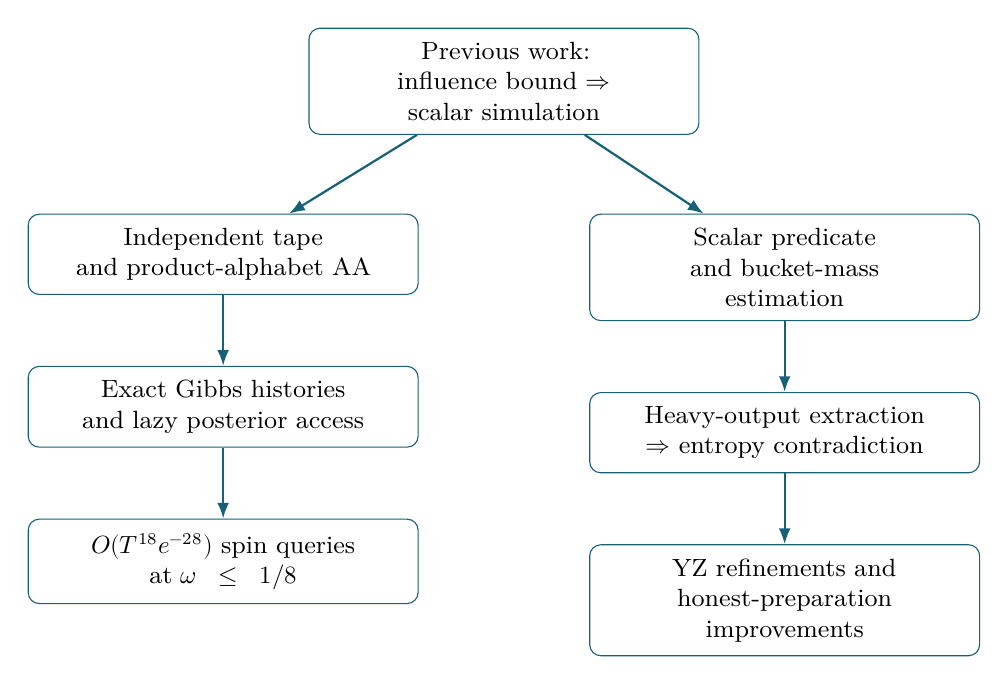
\begin{tikzpicture}[
node distance=9mm and 11mm,
box/.style={draw=Link,rounded corners,align=center,inner sep=5pt,text width=46mm,font=\small},
arr/.style={-{Latex[length=2mm]},draw=Link,thick}]
\node[box] (aa) {Previous work:\\influence bound $\Rightarrow$ scalar simulation};
\node[box,below left=10mm and -14mm of aa] (gibbs) {Independent tape\\and product-alphabet AA};
\node[box,below right=10mm and -14mm of aa] (hash) {Scalar predicate and bucket-mass\\estimation};
\node[box,below=of gibbs] (hist) {Exact Gibbs histories\\and lazy posterior access};
\node[box,below=of hash] (entropy) {Heavy-output extraction\\$\Rightarrow$ entropy contradiction};
\node[box,below=of hist] (gq) {$O(T^{18}e^{-28})$ spin queries\\at $\omega\leq1/8$};
\node[box,below=of entropy] (yz) {YZ refinements and\\honest-preparation improvements};
\draw[arr] (aa)--(gibbs); \draw[arr] (aa)--(hash);
\draw[arr] (gibbs)--(hist); \draw[arr] (hash)--(entropy);
\draw[arr] (hist)--(gq); \draw[arr] (entropy)--(yz);
\end{tikzpicture}
\end{center}

\subsection*{Reading guide and event scope}
Section~\ref{sec:background} gives the problem's known proofs and the external inputs. Sections~\ref{sec:gibbs} and~\ref{sec:distributional} develop the correlated-input arguments; Sections~\ref{sec:certified} and~\ref{sec:yz} develop search and certified randomness. Section~\ref{sec:support} lists the support for each main claim, including the precise scope of Lean verification. Section~\ref{sec:event} separates reported event work from prior work and later preparation. Limitations and open questions are in Section~\ref{sec:open}; tools, human help, and checking procedures are credited in Section~\ref{sec:ai}.

\textbf{Event accounting is not yet final.} The exact start and end of the 40-hour window and the complete contributor list have not been supplied for this revision. The inherited manuscript explicitly attributes Section~\ref{sec:distributional} to Ian Loam's event work. Other activities are listed with their recorded provenance, without counting them as event work until their timing is confirmed. A proof's correctness, its novelty, and its eligibility as event work are separate questions.

\subsection*{Contribution relative to known proofs}
Section~\ref{sec:background} includes a guided sketch of the influential-variable proof as prior work. Turturean's original manuscript reports stronger exponents than the BDST exposition used for our displayed scalar bound \cite{Tur26,BDST26}. Turturean also reports Lean kernel checks of Theorem~1.1 and Corollary~1.2 of that work. We use AA as a proved external theorem. Our separate Lean development verifies selected downstream results; its coverage and remaining hypotheses are stated in Section~\ref{sec:support}.

Our Gibbs contribution is stated precisely in Theorem~\ref{main}. Its constant is dimension-free under $\omega\leq1/8$ and computation is free. It is neither efficient sampling, a full-Dobrushin theorem, nor a polynomial-influence theorem for bounded polynomials on Gibbs measures. Product-alphabet influences below are coordinate-resampling influences, distinct from uniform Boolean flip influence.

Section~\ref{sec:distributional} reports Ian Loam's work on general input laws. Its central result, Theorem~\ref{dist:equivalence}, characterizes failure of acceptance simulation by hard sectors and uses no imported theorem. Its positive results rely on the product-alphabet simulator, and through it on inequality (BC) of \cite{HMP26}. It extends the product and slice transfers of Girish--Mittal--Nehoran--Raz \cite{GMNR26} to arbitrary laws. Its influence-form remark has weaker exponents than \cite{Tur26} and is not claimed as an improvement. Those notes were drafted with the AI assistant Astra and checked by their author lemma by lemma, and the section was condensed with Claude (Anthropic).

Our certified-randomness contributions are Theorems~\ref{heavy}--\ref{sparse}. Yamakawa--Zhandry (YZ) proved the AA-to-entropy route \textbf{conditionally on the AA simulation conjecture} \cite[Theorem 8.4 and Conjecture 8.1]{YZ24}; the 2026 influence proofs supply that hypothesis, which is now a theorem. Our extraction is an alternative factorization through explicit bucket predicates, with explicit exponents, and our coding and honest-preparation refinements are separate inputs. It is not the first use of AA in this setting. Independent work has proved security of the same YZ protocol unconditionally against $o(\log\lambda)$ adaptive quantum queries and against subexponentially many adaptive quantum queries \cite{KRT26,CKMRSST26}. We do not claim to remove an assumption that those works did not already avoid, nor a uniform improvement over their adversary classes. Quantitative comparisons are upper-bound comparisons under one common scalar simulation bound, not optimality claims. Additional comparison and sampling analyses appear in the appendices to keep the main line readable.

% ===== background =====
\section{The problem's known proofs and technical background}\label{sec:background}
This section contains only prior work and the derived scalar conventions needed later. In particular, the proof sketch in Section~\ref{sec:aa-sketch} is an exposition of the recent proof, not a new proof by this paper.

\subsection{Influence, variance, degree, and query algorithms}
For \(x,x'\in\{0,1\}^n\), write \(\Delta(x,x')=\{i:x_i\ne x'_i\}\) and \(x^{\oplus i}\) for \(x\) with bit \(i\) flipped. Unless stated otherwise, expectations on the Boolean cube are uniform. For \(p:\{0,1\}^n\to\mathbb R\), define
\[
 \Var(p)=\E[(p-\E p)^2],\qquad
 \Inf_i(p)=\E\bigl[(p(x)-p(x^{\oplus i}))^2\bigr],\qquad
 \Inf(p)=\sum_i\Inf_i(p).
\]
On \(\{\pm1\}^n\) we write \(\chi_S(x)=\prod_{i\in S}x_i\), and every \(f\) has the Fourier expansion \(f=\sum_S\hat f(S)\chi_S\). A change between the \(\{0,1\}\) and \(\{\pm1\}\) normalizations changes influence by a factor, which will be stated at each use. The acceptance probability of a quantum algorithm making \(q\) queries is a multilinear polynomial of degree at most \(2q\) with values in \([0,1]\) \cite{BBCMW01}.

\begin{example}[Dictator and a two-bit affine polynomial]
For \(p(x)=x_1\), \(\Var(p)=1/4\), \(\Inf_1(p)=1\), and every other influence is zero. For \(p(x)=(x_1+x_2)/2\), \(\E p=1/2\), \(\Var(p)=1/8\), and \(\Inf_1(p)=\Inf_2(p)=1/4\). If the second polynomial is approximated by an influence-guided tree, either coordinate may be queried first. After its value is fixed, the other coordinate remains influential; querying it yields a constant leaf. Thus depth two computes \(p\) exactly, while a one-query leaf returning the mean has a nontrivial residual error.
\end{example}

\begin{example}[Why the degree hypothesis matters]
A single OR does not exhibit the intended phenomenon: \(\mathrm{OR}_n\) has \(\Inf_i=2^{-(n-1)}\), which exceeds its variance. The appropriate contrast is the TRIBES construction. Partition \(w2^w\) coordinates into \(2^w\) blocks of size \(w\), and put
\[
 \mathrm{TRIBES}_w=\mathrm{OR}_{2^w}(\mathrm{AND}_w).
\]
Since a block is all-one independently with probability \(2^{-w}\),
\[
 \Prb[\mathrm{TRIBES}_w=1]=1-(1-2^{-w})^{2^w},\qquad
 \Var(\mathrm{TRIBES}_w)=q_w(1-q_w),
\]
with \(q_w=1-(1-2^{-w})^{2^w}\). For every coordinate,
\[
 \Inf_i(\mathrm{TRIBES}_w)=2^{-(w-1)}(1-2^{-w})^{2^w-1}=2^{-(w-1)}(1-q_w).
\]
The polynomial degree is only \(w\), but as \(w\to\infty\),
\[
 \Var(\mathrm{TRIBES}_w)\to e^{-1}(1-e^{-1})>0,\qquad
 \max_i\Inf_i(\mathrm{TRIBES}_w)\sim2e^{-1}2^{-w}\to0.
\]
Thus substantial variance need not give an influential coordinate when the degree is allowed to grow with \(n\). The influential-variable theorem allows polynomial degradation in inverse degree precisely to exclude this regime from any fixed-degree bound.
\end{example}

A fractional certificate for a real \(p\) at \(x\) is \(\lambda^x\in\mathbb R^n_{\ge0}\) satisfying
\[
 \lambda^x(\Delta(x,y)):=\sum_{i\in\Delta(x,y)}\lambda^x_i\ge|p(x)-p(y)|
\]
for every \(y\). Its cost is \(\|\lambda^x\|_1\), and \(\FC(p)\) is the least uniform upper bound on a family of such costs. For a Boolean \(f\), this says \(\lambda^x(\Delta(x,y))\ge1\) whenever \(f(x)\ne f(y)\).

\subsection{The influential-variable theorem}
\begin{theorem}[Bounded low-degree functions have influential variables]\label{thm:aa}
For every polynomial \(p:\{0,1\}^n\to[0,1]\) of degree at most \(d\ge1\) with \(\Var(p)>0\),
\[
 \max_i\Inf_i(p)\ge\Omega\Bigl(\frac{\Var(p)^8}{d^{12}}\Bigr)
\]
in the \(\{0,1\}\) convention above. The implied constant is absolute. Constant functions are the \(d=0\) or \(\Var(p)=0\) case and need no influence lower bound.
\end{theorem}
This is the form given by Blanc, Docter, Strassle, and Tan \cite[Theorem~1]{BDST26}. Equivalently, the original AA assertion is: if \(\Var(p)\ge\eta>0\), then \(\max_i\Inf_i(p)\ge(\eta/d)^{O(1)}\) \cite[Conjecture~6 (arXiv version)]{AA14}. It does not assert an exponent 7; that stronger conclusion comes from Turturean's separate normalization below. Turturean's original manuscript \cite{Tur26} states the stronger form on \(\{\pm1\}^n\) for \(f:\{\pm1\}^n\to[-1,1]\) of degree at most \(d\ge1\):
\[
 \max_j\E\biggl[\Bigl(\frac{f(x)-f(x^{\oplus j})}{2}\Bigr)^2\biggr]\ge\frac{\sqrt{15}}{500\pi^4}\,\frac{\Var(f)^{5/2}}{d^6}.
\]
To connect normalization explicitly, set \(f=2p-1\) for \(p:\{0,1\}^n\to[0,1]\). Then
\[
 \Inf^{\mathrm{Tur}}_j(f)=\Inf_j(p),\qquad \Var(f)=4\Var(p).
\]
Calling the latter influence \(\Inf^{\mathrm{AA}}_j\) shows that the same quantity is being measured. The original \(0/1\) bound has constant \(8\sqrt{15}/(125\pi^4)\), exactly 32 times the \(\pm1\) constant displayed above; it reads
\[
 \Inf^{\mathrm{AA}}_i(p)\ge\frac{8\sqrt{15}}{125\pi^4}\,\frac{\Var(p)^{5/2}}{d^6}\ge\Bigl(\frac{\Var(p)}{d}\Bigr)^7
\]
in Turturean's Corollary~1.2. The comparison is meaningful only after this normalization step. We instead use BDST's weaker \(\Var^8/d^{12}\) form consistently in the scalar calculation, because it is the form supplied by the hashing analysis. Substituting a stronger theorem can improve upper bounds without changing qualitative claims.

The original manuscript and repository specifically report Lean kernel checks of Turturean's Theorem~1.1 and Corollary~1.2 \cite{Tur26}. That external verification does not establish the downstream results automatically. Section~\ref{sec:support} separately records which downstream components have been checked in our Lean development and which assemblies remain written proofs only.

\subsection{The traditional proof of the influence bound: a guided sketch}\label{sec:aa-sketch}
There are four conceptual steps: low-degree fractional certificates; a certificate--influence inequality for Boolean functions; routing lemmas that prove the latter; and thresholding to pass from Boolean functions back to \(p\). The determinant and certificate-complexity inputs are the most technical parts of the source proof and are cited rather than secretly reproved.

\paragraph{The obstacle.}
For ordinary certificates, two bichromatic inputs force an intersecting certificate, giving overlap at least one and allowing the usual Poincaré path argument. Fractional certificates need not intersect at all. With flat vectors \((2/n,\ldots,2/n)\) at the all-zero and all-one inputs of Majority, their inner product is only \(\sum_i(2/n)^2=4/n\), so the non-intersection premise is gone. Routing is therefore not optional machinery: it supplies the substitute for the missing intersection fact while preserving monochromatic faces.

\paragraph{1. Bounded low degree gives cheap fractional certificates.}
Agarwal and Ben--David's fractional block-sensitivity theorem implies
\[
 \FC(p)=O(d^2)
\]
for every degree-\(d\) polynomial \(p:\{0,1\}^n\to[0,1]\) \cite[Fact~2.4 and the cited ABD result]{BDST26}. This is the only step in the BDST presentation that uses bounded polynomial degree. The remainder applies to any function with small fractional certificate complexity.

\paragraph{2. Cheap certificates give an influential coordinate after Booleanization.}
For a nonconstant Boolean \(f\) and any choice of fractional certificates \(\{\lambda^x\}\), define
\[
 R_1=\E_x\Bigl[\frac{\mathbf 1\{f(x)=1\}}{\|\lambda^x\|_1}\Bigr],\qquad
 R_0=\E_y\Bigl[\frac{\mathbf 1\{f(y)=0\}}{\|\lambda^y\|_1}\Bigr].
\]
The certificate--influence inequality \cite[Lemma~2.5]{BDST26} is
\[
 \max_i\Inf_i(f)\ge4R_1R_0.
\]
It is sharp for a dictator. A worst-case certificate-cost bound would not be robust enough for the next thresholding step: dividing by \(|p(x)-t|\) makes individual certificates arbitrarily expensive, while the two averages remain controllable.

\paragraph{3. Routing proves the certificate--influence inequality.}
Write \(A=f^{-1}(1)\). For positive weights \(w\), define the overlap of two certificates on the differing coordinates by
\[
 \mathrm{overlap}_{w,\Lambda}(x,y)=\sum_{i\in\Delta(x,y)}w_i\lambda^x_i\lambda^y_i.
\]
The weighted all-pairs lemma \cite[Lemma~2.8]{BDST26} reads
\[
 \sum_i\frac{\Inf_i(A)}{w_i}\ge4\E_{x,y}\Bigl[\frac{\mathbf 1\{x\in A,y\notin A\}}{\mathrm{overlap}_{w,\Lambda}(x,y)}\Bigr],
\]
with the right-hand ratio taken as zero off bichromatic pairs. Specializing weights according to normalized certificate masses and applying Cauchy--Schwarz gives \(4R_1R_0\).

The all-pairs lemma is a consequence of the routing lemma \cite[Lemma~2.10]{BDST26}. If \(T\) is a monochromatic face of \(x\in A\), then every bichromatic \((x,y)\) can be assigned \(z\in A\cap\mathrm{cube}(x^{\oplus T},y)\) such that, coordinate by coordinate,
\[
 \Prb[x\in A,y\notin A,z_i\ne y_i]\le\tfrac14\Inf_i(A).
\]
To see the connection with overlap, put heavy coordinates of \(\lambda^y\) into \(T\), with heaviness threshold equal to the overlap. The \(\lambda^x\)-mass of \(T\) is then less than one, so \(T\) remains monochromatic. Every route from \(y\) back to \(A\) must use many light coordinates: if each has mass at most \(\tau\), unit fractional-block sensitivity forces at least \(1/\tau\) of them. Routing therefore turns coordinate influence into a lower bound for reciprocal overlap.

The antipodal routing lemma \cite[Lemma~2.11]{BDST26} proves the routing statement inside every subcube and loses only a further factor \(1/2\). When \(y=\bar x\), it produces \(z\in A\cap\mathrm{cube}(x^{\oplus T},\bar x)\) with \(\Prb[x\in A,z_i\ne\bar x_i]\le\Inf_i(A)/2\). Applying it separately to antipodal subcubes and averaging gives the displayed \(1/4\).

The face constraint is the real difficulty. The proof writes two matrices \(M\) and \(M_T\), indexed by \(A\), in formal variables \(\zeta_i\). Terms in \(\det M\) record the number of coordinates in which a permutation \(\pi:A\to A\) fails to reach the antipode; terms in \(\det M_T\) retain only permutations respecting every designated face. The determinant-equivalence lemma \cite[Lemma~2.16]{BDST26} states that these two determinant polynomials have exactly the same Pareto-minimal monomials. Its representative algebraic input is a row identity, for each monochromatic face \(T(x)\),
\[
 \Bigl(\prod_{i\in T(x)}(1-\zeta_i^2)\Bigr)\mathrm{row}_x(M_T)=\sum_{S\subseteq T(x)}\Bigl(\prod_{i\in S}(-\zeta_i)\Bigr)\mathrm{row}_{x^{\oplus S}}(M).
\]
The rows on the right exist because \(T(x)\) is monochromatic. Pareto degrees control the coordinatewise error. We cite the full determinant argument from \cite[Sections~2.5 and~3]{BDST26}; merely invoking nonvanishing determinants would not establish the required degree bounds.

\paragraph{4. Threshold averaging proves AA.}
For nonconstant \(p\), let \(\mu=\E p\) and \(\sigma=\E|p-\mu|\), and set \(p_t(x)=\mathbf 1\{p(x)>t\}\). For every \(t\) outside the finite set \(\{p(x):x\in\{0,1\}^n\}\), the vector \(\lambda^x/|p(x)-t|\) is a fractional certificate of \(p_t\) at \(x\); this finite set has Lebesgue measure zero and is avoided by averaging \(t\) over an interval. For one fixed \(t\), the event \(p(x)=t\) need not be null on the cube. The certificate--influence inequality gives
\[
 \max_i\Inf_i(p_t)\ge\Omega\Bigl(\frac{\E(p-t)_+\,\E(t-p)_+}{\FC(p)^2}\Bigr).
\]
For \(t\in[\mu-\sigma/4,\mu+\sigma/4]\), each expectation in the numerator is at least \(\sigma/4\), so the right side is \(\Omega(\sigma^2/\FC(p)^2)\). On the other hand, a window-jump decomposition for \(\theta>0\) gives
\[
 \max_i\Inf_i(p_t)\le2\Prb[t<p(x)\le t+\theta]+\frac{\max_i\Inf_i(p)}{\theta^2}.
\]
Averaging \(t\) uniformly over an interval of length \(\sigma/2\) bounds the expectation of the first term by \(4\theta/\sigma\). If \(M=\max_i\Inf_i(p)\), then
\[
 \frac{M}{\theta^2}+\frac{4\theta}{\sigma}\ge\Omega(\sigma^2/\FC(p)^2)
\]
for every \(\theta>0\). Choosing \(\theta=(\sigma M)^{1/3}\) yields
\[
 M\ge\Omega(\sigma^8/\FC(p)^6).
\]
Finally \(\FC(p)=O(d^2)\) and \(\sigma\ge\Var(p)\) for \(0\le p\le1\) prove Theorem~\ref{thm:aa}. This final polynomial loss is a consequence of the deliberately unoptimized BDST presentation, not a claim that its exponents are optimal.

\subsection{From influence to scalar simulation}
We now derive the exact coarse scalar convention used throughout the application sections. The proof is the AA potential argument with explicit parameters \cite{AA14,BDST26}.

\begin{theorem}[Most-oracle deterministic scalar estimator]\label{thm:scalar}
Let \(\mc B\) be a Boolean-output quantum algorithm making at most \(q\) bit queries to a Boolean table \(H\in\{0,1\}^N\). For every \(N\) and every \(0<e,\delta<1\) there is a deterministic classical estimator \(E_{\mc B}\) such that
\[
 \Prb_H\bigl[|E^H_{\mc B}-\Prb[\mc B^H=1]|>e\bigr]\le\delta.
\]
Its number of oracle queries is at most
\[
 F(q,e,\delta)=O((q+1)^{13}e^{-16}\delta^{-9}),
\]
uniformly in \(N\). The inner probability is over \(\mc B\)'s measurement randomness on a fixed \(H\); the outer probability is over uniformly random oracle tables. At every completed leaf \(E_{\mc B}\) returns the exact conditional mean over all completions of the unread bits, chosen by deterministic free computation rather than sampling.
\end{theorem}
\begin{proof}
Let \(D=\max\{1,2q\}\) and let \(p_H\) be the acceptance polynomial. Every restriction has degree at most \(D\) and values in \([0,1]\). Using Parseval and boundedness, its total influence satisfies
\[
 \Phi(p)=\Inf(p)=4\sum_S|S|\hat p(S)^2\le4D\Var(p)\le D.
\]
When coordinate \(i\) is queried and then its value \(X_i\) is drawn uniformly, the exact potential identity in this convention is
\[
 \Phi(p)-\E_{X_i}\Phi(p|_{X_i})=\Inf_i(p).
\]
Indeed \(\Inf_i(p)=4\sum_{S\ni i}\hat p(S)^2\) and \(\Phi=4\sum_S|S|\hat p(S)^2\). Averaging the restriction subtracts exactly one unit of degree weight for every \(S\) containing \(i\), so the drop is \(4\sum_{S\ni i}\hat p(S)^2=\Inf_i(p)\), including the outer factor of 4. Set \(\tau=e^2\delta/2\). If \(\Var(p)>\tau\), Theorem~\ref{thm:aa} supplies a coordinate with influence \(\Omega(\tau^8/D^{12})\). Follow that coordinate with a fixed tie-breaking rule and recurse, stopping if the current variance is at most \(\tau\). Optional stopping applied to the nonnegative potential gives expected depth \(O(D^{13}\tau^{-8})=O(D^{13}e^{-16}\delta^{-8})\). Truncate at \(2/\delta\) times this expectation; Markov contributes failure at most \(\delta/2\).

At every nontruncated leaf, variance is at most \(\tau\), and the algorithm returns the mean of \(p\) over all completions of the unread bits. Chebyshev bounds the probability of error exceeding \(e\) by \(\Var(p)/e^2\le\delta/2\). The two failure modes add to \(\delta\), and the cap contributes one further factor \(\delta^{-1}\). Computing the mean and selecting coordinates is free in the query model.
\end{proof}

\begin{remark}[Error conventions]
Theorem~\ref{thm:scalar} gives an estimate with small error on most oracles. The Gibbs theorem instead bounds \(\E_\mu|D-Q|\) over an input law, with no inputwise guarantee. The product-alphabet resampling influence used later is \(\Prb[G(X)\ne G(X_{-i},X'_i)]\), not the squared flip influence used in this section. Keeping these notions separate is essential to all parameter claims.
\end{remark}

\subsection{Boolean presampling: the precise bit-fixing formulation}
A \(P\)-bit-fixing distribution over oracles \(O:[N]\to\{0,1\}\) fixes at most \(P\) coordinates to chosen values and leaves every other coordinate independent and uniform. The relevant theorem concerns mixtures of these distributions and all distinguishers simultaneously, not merely a single convenient restriction.

Let \(U_N\) be uniform on \(\{0,1\}^N\), let \(F:\{0,1\}^N\to\{0,1\}^S\) produce \(S\)-bit advice, and let \(\mathbb A\) take \(S\) input bits and make at most \(T\) oracle queries. The Boolean presampling statement asks for constants \(C\) and a function \(h(S)\), independent of \(N,F,P,T,\mathbb A\), such that for every \(P\ge1\) there are \(P\)-bit-fixing mixtures \(\{Y_z\}_{z\in\{0,1\}^S}\), depending on \(F\) and \(P\) but not on \(T\) or \(\mathbb A\), for which
\[
 \Bigl|\Prb_{O\sim U_N}[\mathbb A^O(F(O))=1]-\Prb_{\substack{Z\sim F(U_N)\\\tilde O\sim Y_Z}}[\mathbb A^{\tilde O}(Z)=1]\Bigr|\le h(S)\Bigl(\frac CP\Bigr)^T
\]
for every \(T\) and \(\mathbb A\) simultaneously. This exponential-in-\(T\) formulation is LM26's strengthening of GLLZ's general \((2,N)\)-oracle presampling statement, whose bound has polynomial form \(h(S)\,T(\log2/P)^C\) \cite[Conjecture~4]{GLLZ21}; for Boolean oracles, \(\log2=1\). The simulation-to-strong-presampling implication is \cite[Theorem~5.7]{LM26}. The reverse direction uses the original GLLZ argument (their Theorem~4: Conjecture~4 implies Conjecture~3 and then Conjecture~1) \cite{GLLZ21}. Unrestricted growth of \(h(S)\) is permitted and does not obstruct the equivalence.

The decision tree behind Theorem~\ref{thm:scalar} also yields an explicit \emph{conditional-mean restriction statement}, not just the simultaneous mixture above. Its returned leaf mean is an expectation of the acceptance polynomial under a bit-fixing law with all unread coordinates set to zero (or any other fixed assignment).

\begin{proposition}[A restriction with a biased conditional mean]\label{prop:restriction}
Let \(f\) be the acceptance polynomial of a \(q\)-query Boolean-oracle algorithm and let \(v=\Var(f)>0\). There are \(J\subseteq[N]\) and an assignment \(x_J\in\{0,1\}^J\) such that
\[
 |J|\le C_F2^{93}(q+1)^{13}v^{-34},\qquad
 \bigl|\E_{x'_{\bar J}}f(x_J,x'_{\bar J})-\E f\bigr|\ge\frac{3v}4,
\]
where \(C_F\) is the absolute constant hidden in the query bound \(F(q,e,\delta)\) for Theorem~\ref{thm:scalar}.
\end{proposition}
\begin{proof}
Apply Theorem~\ref{thm:scalar} with error \(e=v/8\) and exception \(\delta=v^2/32\). The tree deterministically returns some conditional mean \(g(x)=f(x_{J(x)},0_{\bar J(x)})\) at depth at most \(F(q,v/8,v^2/32)\). On the event \(|f(x)-g(x)|\le e\) the \(\ell_2\) error is at most \(e^2\), and the exceptional event has mass at most \(\delta\), with both \(f,g\) in \([0,1]\). Hence
\[
 \|f-g\|_2^2\le e^2+\delta=\frac{3v^2}{64},\qquad \E|f-g|\le\frac v4.
\]
Set \(\bar f=\E f\). By the sign of the difference between expectations and the law of total expectation,
\[
 \E|g-\bar f|\ge\E[(f-\bar f)^2]-\E|g-f|\ge v-\frac v4=\frac{3v}4.
\]
Choose a leaf attaining this lower bound. Since \(8^{16}32^9=2^{48}2^{45}=2^{93}\), the number of queries along its branch is bounded by \(F(q,v/8,v^2/32)\), which is the advertised bound.
\end{proof}

\begin{proposition}[Smoothness corollary]
Let \(\eta>0\) and suppose that whenever \(|J|\le C_F6^{16}18^9(q+1)^{13}\eta^{-34}\), every assignment \(x_J\) satisfies \(|\E_{\bar J}f(x_J,x'_{\bar J})-\E f|\le\eta\). Then \(\Var(f)\le4\eta/3\).
\end{proposition}
\begin{proof}
If \(v>4\eta/3\), then \(v/8>\eta/6\) and \(v^2/32>\eta^2/18\). Monotonicity of \(F\) gives a copy of Proposition~\ref{prop:restriction} with \(|J|\le C_F6^{16}18^9(q+1)^{13}\eta^{-34}\), and its deviation \(3v/4>\eta\) contradicts the hypothesis. The variance cannot exceed \(4\eta/3\).
\end{proof}

The same \(\ell_2\)-restriction argument is used in GLLZ's Appendix~B (Theorem~10 and its smoothness discussion); the explicit exponents here are just what results from \(F\) \cite{GLLZ21}. This says nothing about computational efficiency: exact conditional means are free in the query model but potentially expensive to compute. Nor does one restriction mean that every input is easy, nor is this a product-alphabet statement, nor is the mixture/presampling equivalence identical to the polynomial-influence conjecture.

The leaf interpretation also explains the simultaneous statement: conditioned on advice and a transcript, the unread oracle coordinates have a bit-fixing law, and the returned leaf mean is an acceptance expectation under that law. The standard mixing argument produces the relevant mixtures \cite[Theorem~5.7]{LM26}. No claim is made that one pointwise restriction approximates every input at once. With the influential-variable theorem now proved, the simulation and presampling formulations are statements rather than conjectures, subject to the cited response-alphabet and advice hypotheses.

\subsection{Prior distributional and certified-randomness results}
Girish--Mittal--Nehoran--Raz studied AA under biased product inputs and fixed-Hamming-weight slices, proving equivalences to the uniform formulation for fixed bias parameters \cite{GMNR26}. These results are the conceptual product-law endpoint motivating our Gibbs branch; they are different from the arbitrary-alphabet, arbitrary-marginal theorem proved directly in Section~\ref{sec:gibbs}. A fixed-bias equivalence should not be silently generalized to all marginals or to correlated laws.

Yamakawa--Zhandry constructed a folded Reed--Solomon search relation for which efficient quantum generation and verification coexist with exponential classical query hardness \cite{YZ24}. Their Theorem~8.4 proves an AA-to-certifiable-min-entropy implication \textbf{conditionally on the AA simulation conjecture} \cite[Conjecture~8.1 and Theorem~8.4]{YZ24}. The 2026 influential-variable proofs discharge that antecedent; in our bit-oracle setting, Theorem~\ref{thm:scalar} makes the required query polynomial explicit. Function-oracle formulations with answer length \(m\) also carry the corresponding \(m\)-dependence discussed in YZ's Remark~6. The displayed YZ extraction repeatedly runs the prover, estimates frequencies, randomly chooses a cutoff and a canonical heavy valid output, and simulates its output bits. Sections~\ref{sec:certified} and~\ref{sec:yz} preserve this attribution and unpack the construction before comparing it with our direct hash-and-verify alternative.

Two subsequent papers eliminate the AA assumption in different adversary regimes without relying on it: Khurana--Roberts--Tal covers \(o(\log\lambda)\) adaptive queries \cite{KRT26}, and Coladangelo et al.\ covers subexponentially many adaptive queries \cite{CKMRSST26}. We do not use those results as inputs and do not claim priority for unconditional security of the YZ protocol. Comparisons here concern a different extraction mechanism and explicit entropy parameters, not an across-the-board strengthening of those works.

For the Gibbs application below, Harrow--Wei's adaptive quantum simulated annealing uses Markov chains with Gibbs stationary distributions at successive temperatures, produces qsamples, employs amplitude estimation, and applies the framework to partition functions and Bayesian inference \cite{HW20}. We use only this algorithmic context, not its performance guarantees.

% ===== gibbs_intro =====
\section{Mean simulation on high-temperature Gibbs inputs}\label{sec:gibbs}
The uniform and biased-product results assume independence that physical and probabilistic models often lack. A direct density comparison between a Gibbs law and a product law generally loses an exponential factor in dimension, so it cannot prove an \(n\)-independent query theorem. This section instead retains independence in a latent history and uses Bayes-exact posterior access to answer queries on the physical configuration.

\subsection{Motivation: a controlled departure from independence}
Let
\[
 H(x)=-\sum_{|A|\ge2}J_A\prod_{i\in A}x_i-\sum_ih_ix_i,\qquad
 \mu_\beta(x)=\frac{e^{-\beta H(x)}}{Z_\beta},\qquad x\in\{\pm1\}^n.
\]
At \(\beta=0\), every coordinate is independent and uniform. Small weighted interaction strengths give a product-like regime, whereas larger inverse temperature can make interactions dominant and can concentrate the law on a highly constrained ground-state set. Gibbs families therefore provide an explicit, parameterized way to investigate how much independence an AA-style simulation actually needs. This is not a literal interpolation through every distribution, and no claim is made that every measure of correlation increases monotonically.

The endpoint distinction is genuine. Product-distribution variants of AA work under the previously cited hypotheses and the product-alphabet machinery below. By contrast, dimension-free polynomial-influence AA cannot hold for all Gibbs laws with a constant uniform in \(\beta\). Consider the all-to-all three-spin Hamiltonian \(H_3=-J(x_1x_2+x_2x_3+x_3x_1)\) with \(J>0\), put \(u=e^{-\beta J}\), and let \(p=\mathrm{MAJ}_3\) with values in \(\{0,1\}\). An exact enumeration gives
\[
 \Var_{\mu_\beta}(p)=\frac14,\qquad
 \Inf_i^{\mu_\beta}(p)=\frac{2u^4}{1+3u^4},\qquad
 \Prb_{\mu_\beta}[x\in\{+++,---\}]=\frac1{1+3u^4}.
\]
The influence is positive at every finite \(\beta\) but tends to zero, while the variance remains \(1/4\). The zero-temperature law here means the weak limit uniform on \(\{+++,---\}\), not \(\mu_\beta\) at finite \(\beta\): on that limit law every flip influence is exactly zero. For this model \(\omega=2\beta J\), so \(\omega\le1/8\) requires \(\beta J\le1/16\); the low-temperature obstruction is outside our hypothesis. It is also not an obstruction to every mean query-simulation statement. On the known two-point ground support, one spin query identifies the configuration and free computation returns \(Q(x)\) exactly. The obstruction is specifically to a uniform flip-influence bound, and it explains why the theorem uses history structure rather than transporting product polynomial-influence AA directly.

Our parameter is
\[
 \omega=\beta\max_i\sum_{A:\,i\in A,\,|A|\ge2}(|A|-1)|J_A|.
\]
The condition \(\omega\le1/8\) is a sufficient high-temperature condition, not a characterization of every Dobrushin-unique model. It controls the local heat-bath updates strongly enough that their conditional means can be exactly randomized by signed parities or constants with contracting expected supports. Local updates then generate the correlated configuration without requiring a global product density bound. This is the conceptual bridge: \textbf{independence is recovered in the update history, not claimed for the physical spins.} ``High temperature'' here must not be read as an efficient-mixing or easy-sampling theorem. We charge queries, while computation and storage are free.

\subsection{An instructive application: annealing and partition functions}
Partition-function and free-energy calculations offer a concrete reason for a quantum algorithm to process Gibbs-distributed inputs. Set \(Z(\beta)=\sum_xe^{-\beta H(x)}\). If \(\beta_\ell<\beta_{\ell+1}\), then
\[
 \frac{Z(\beta_{\ell+1})}{Z(\beta_\ell)}
 =\sum_x\frac{e^{-\beta_\ell H(x)}}{Z(\beta_\ell)}e^{-(\beta_{\ell+1}-\beta_\ell)H(x)}
 =\E_{x\sim\mu_{\beta_\ell}}\bigl[e^{-\Delta\beta_\ell H(x)}\bigr],
\]
where \(\Delta\beta_\ell=\beta_{\ell+1}-\beta_\ell\ge0\). Thus each annealing step is a mean of a bounded positive quantity under the current Gibbs law. Shifting \(H\) by its minimum makes \(H'=H-\min H\ge0\) and makes the quantity a \([0,1]\)-valued acceptance function through a controlled rotation or equivalent postprocessing; the known shift factor must be carried when reconstructing \(Z\). Products of the exact ratios, together with an easy initial value such as \(Z(0)=2^n\), algebraically reconstruct a final partition function and hence \(\log Z\) or a suitably normalized free energy. Quantum simulated-annealing algorithms use precisely this combination of Gibbs stationary laws, quantum samples, and amplitude estimation in a larger program \cite{HW20}.

There is an important error-type caveat. Theorem~\ref{main} supplies additive mean error \(e\) on an acceptance ratio, not multiplicative error on a partition function. If \(R_\ell\ge r>0\) for \(K\) stages and each stage is estimated absolutely to within \(e\), the elementary product bound gives relative error at most \((1+e/r)^K-1\) in \(\prod_\ell R_\ell\). A small ratio floor or a separate averaging/confidence protocol is therefore needed before making any multiplicative estimate of \(Z\) or additive estimate of \(\log Z\). No such stage-ratio lower bound or confidence amplification is proved here. This paragraph supplies an input-model illustration, not a new partition-function algorithm or a cost comparison with the coherent qsamples and spectral-gap assumptions used by \cite{HW20}.

If a stage satisfies \(\omega\le1/8\) and a quantum routine implements such acceptance with \(T\) physical-spin oracle queries, Theorem~\ref{main} gives a deterministic classical baseline for its mean acceptance, with error \(e\) and \(O(T^{18}e^{-28})\) spin queries. This is a structural match between an application and a theorem, not a new partition-function algorithm. Evaluating a global Hamiltonian can require many spin queries; thermal-state or qsample preparation is not supplied or charged; and the simulator's computation is unrestricted. We therefore claim no total-runtime improvement, quantum advantage, or replacement for Gibbs-state preparation. At most, this illustrates why query-only mean approximation on correlated thermal inputs is useful for benchmarking and for understanding the input-oracle component of such algorithms.

\subsection{Logical structure of the proof}
The proof has two independent modules and one transfer lemma.
\begin{enumerate}
\item \textbf{Bayes-exact histories.} Lemma~\ref{lem:maps} constructs sparse random update maps. Lemma~\ref{lem:stationary} gives exact stationary histories and map disintegration. Lemma~\ref{lem:discrepancy} proves forward discrepancy \(\vartheta^L\) by path counting, and Lemma~\ref{lem:work} bounds posterior work by \(O(s)\) for a source tree of depth \(s\).
\item \textbf{Product-alphabet AA.} An alphabet-free quantum adversary bound produces fractional certificates. A product certificate--influence inequality and influence-guided querying give a deterministic source tree, and thresholding yields real-valued simulation.
\item \textbf{Transfer.} The physical acceptance function is compared with a truncated source algorithm by the recursive norm estimate of Lemma~\ref{lem:hybrid}. The same source tree is used for every physical input, with source symbols supplied by the exact posterior sampler. The errors are allocated \(e/3\) each in Theorem~\ref{main}.
\end{enumerate}
In this section only, \(n\) is the number of spins and \(L\) the number of sweeps. Certified-randomness sections use separate output-length and code parameters when there is a risk of confusion. A source is \(\Omega=\prod_i\Omega_i\) with law \(\nu=\bigotimes_i\nu_i\). Quantum symbol oracles are controlled unitaries; an oracle difference has norm at most two, not a norm proportional to a symbol distance. Pre-query weights \(q_{r,i}\) are squared projection norms, equivalently coordinate-query probabilities, so \(\sum_iq_{r,i}\le1\); bare projection norms are not used. Classical queries return whole symbols, while computation and preprocessing are free. The final error is mean absolute error over the physical input, not conditional accuracy for each input.

% ===== gibbs_core =====
\subsection{Local Gibbs and oracle conventions}
Let \(\beta\ge0\), \(J_A,h_i\in\mathbb R\) be finite and let
\[
 H(x)=-\sum_{A\subseteq[n],|A|\ge2}J_A\prod_{i\in A}x_i-\sum_ih_ix_i,\qquad
 \mu_\beta(x)=Z_\beta^{-1}e^{-\beta H(x)},
\]
with \(Z_\beta=\sum_{y\in\{\pm1\}^n}e^{-\beta H(y)}\). Since all coefficients are finite, \(\mu_\beta(x)>0\) for every \(x\). Define the local field and its Fourier statistics
\[
 u_i(\eta)=\beta\sum_{A\ni i,|A|\ge2}J_A\chi_{A\setminus\{i\}}(\eta),\qquad
 \chi_S(\eta)=\prod_{j\in S}\eta_j,\qquad
 \|f\|_A=\sum_S|\hat f(S)|,\qquad
 W(f)=\sum_S|S||\hat f(S)|.
\]
Here \(\hat f(S)\) is the ordinary \(\pm1\)-Fourier coefficient. I use \(A\) both for the interaction support and for the norm subscript; they should not be confused. Set
\[
 K_i:=\beta\sum_{A\ni i,|A|\ge2}|J_A|,\qquad
 w_i:=\beta\sum_{A\ni i,|A|\ge2}(|A|-1)|J_A|,\qquad
 \omega:=\max_iw_i.
\]
Since \(\|u_i\|_A\le K_i\) and \(W(u_i)\le w_i\), and \(|A|-1\ge1\), the hypothesis \(\omega\le1/8\) forces \(K_i,w_i\le1/8\) for every \(i\). Substituting fixed spins for some coordinates cannot increase these bounds. The external field \(\beta h_i\) can be arbitrary.

Fix one finite graph: put \(N_i=\bigcup_{A\ni i,|A|\ge2}(A\setminus\{i\})\), its size unrestricted. At site \(i\), the actual conditional spin law is
\[
 p_i(y\mid\eta)=\frac{1+y\tanh(\beta h_i+u_i(\eta))}{2},\qquad y\in\{\pm1\}.
\]
This is the resampling step used below. A full sweep updates spins in the fixed order \(1,\ldots,n\) once each. Event \((\ell,i)\) means the update of site \(i\) during sweep \(\ell\in[L]\). The order is \(\ell\), then \(i\); no coloring argument is used.

\subsubsection{Quantum source oracles, classical queries and the error convention}
For finite alphabets \(\Omega_i\), a source is \(\Omega=\prod_i\Omega_i\) with law \(\nu=\bigotimes_i\nu_i\). A quantum query acts on a designated query register and workspace by a unitary controlled by the input symbol. Equal symbols cause equal unitary calls. If \(V_i(a)\) is arbitrary unitary, a convenient form is \(\sum_i|i\rangle\langle i|\otimes V_i(\omega_i)\). A unitary symbol oracle difference has operator norm at most 2, not a norm proportional to the symbol distance. Such an oracle family includes phase oracles, permutations and suitable cyclic-data queries. An algorithm includes fixed workspace unitaries between queries and a final measurement \((P_{\mathrm{acc}},I-P_{\mathrm{acc}})\), giving \(0\le Q(x)=\langle\psi_x|P_{\mathrm{acc}}|\psi_x\rangle\le1\).

For \(q_{r,i}(x)\) I use the squared norm of the projection of the purified state onto the branch that queries coordinate \(i\) immediately before step \(r\); equivalently it is the probability of querying coordinate \(i\) at that step, and in particular \(\sum_iq_{r,i}(x)\le1\). The bare norm is not used. Purification is used when overlap is needed. Classical symbol queries return an entire symbol. Reading a map, arithmetic, lookup tables, Bayes-normalisation, computing a conditional field, choosing a decision-tree coordinate, and storing trees are free. Computation and preprocessing are free; only physical spin queries are ultimately charged.

The final target is: \textbf{worst-case bounded queries, mean error over the physical input}, not an error bound conditional on every input. \(T\) denotes query number and \(T\ge1\), and the error parameter satisfies \(0<e<1\). A quantum query algorithm (including its purified states and query weights) is part of the input data, not merely the functional value \(Q(x)\).

\subsubsection{Sweep history and prior maps}
At event \(e=(\ell,i)\) let \(\eta_e\) be the assignment of \(N_i\) immediately before the event, and \(y_e\) the resulting spin after the event. A prior event map law \(\nu_e\) will be independent across events before any trajectory is conditioned. Given output \(y\), define
\[
 \nu_e^{(\eta,y)}(m)=\frac{\nu_e(m)\mathbf 1[m(\eta)=y]}{p_e(y\mid\eta)},\qquad
 p_e(y\mid\eta)=\sum_m\nu_e(m)\mathbf 1[m(\eta)=y],
\]
whenever \(p_e(y\mid\eta)>0\). In the intended Gibbs trajectory, positivity follows from finite coefficients and full support of \(\mu_\beta\). We use two time indexings. At sweep granularity, \(Y^\ell\) is the configuration after \(\ell\) complete sweeps, with \(Y^0\) stationary and \(Y^L=X\). For local recursions, flatten the events to \(\tau(\ell,i)=(\ell-1)n+i\in\{1,\ldots,nL\}\), and let \(W^\tau\) be the configuration after the first \(\tau\) events. Thus \(W^{\ell n}=Y^\ell\), \(W^0=Y^0\), and \(W^{nL}=X\). A source event at flattened time \(t_e\) has resulting spin \(y_e=W^{t_e}_{i(e)}\) and neighbour vector \(\eta_e=W^{t_e-1}_{N_{i(e)}}\).

\subsubsection{Dependency conventions}
For a prior map tape \(Z=(M_e)\), define \(F_L(Z)\) by starting from the all-plus configuration and applying the maps \(M_e\) in chronological order through \(L\) sweeps. In the coupling below, the true trajectory instead starts from a stationary \(W^0\) and uses the same tape; its final configuration is \(X\).

The autoregressive evaluation of a spin of \(F_L(Z)\) starts at its last update. For a non-boundary event \((\ell,i)\) and each \(j\in S(M_{\ell,i})\), the child is the most recent update of \(j\) strictly before the parent, or a boundary leaf if no such event exists. The underlying event's map is shared if it is reached on different node-paths, but different paths still count separately in the proof. Repeated children, map sharing, caching and stopping at a finite number of vertices are all permitted: nothing requires events to be globally unique.

The final truncated evaluator \(F_{L,B}\) is defined query by query: for each root coordinate \(i\), breadth-first traversal uses its own hard cap of \(B\) symbol reads (cache hits cost no new read); no cap is shared between two root queries. By default, when fully traversed it returns the same answer as \(F_L\). Once the cap would be exceeded, it returns the preassigned constant \(+1\) for that \emph{root query}, discarding the partial evaluation. This discarding convention is used consistently and avoids referring to unvisited maps. Reversible uncomputation costs at most another \(B\) map reads. It differs from \(F_L\) only if the full unrolled tree for that root has more than \(B\) vertices.

\subsection{Exact update maps, stationary histories, and posterior work}
\begin{lemma}[Exact sparse update maps]\label{lem:maps}
Suppose \(m(\eta)=\tanh(\beta h_i+u(\eta))\), where \(u\) has no constant Fourier term, \(\|u\|_A\le K\le1/8\), and \(W(u)\le w\le1/8\). There is a random map \(M\), either constant or a signed parity, whose law is fixed by the site's data \((\beta h_i,u)\) and is independent of \(\eta\), such that \(\E M(\eta)=m(\eta)\) for every \(\eta\). Its support obeys, for each fixed \(\eta,y\) with \(p(y\mid\eta)>0\),
\[
 \E|S(M)|\le\vartheta\,p(y\mid\eta),\qquad
 \frac{\E|S(M)|}{p(y\mid\eta)}\le\vartheta:=\frac{160}{169}<1.
\]
In particular, an unconditioned fresh prior map has \(\E|S(M)|\le80/169\).
\end{lemma}
\begin{proof}
Let \(r=\tanh\beta h_i\), \(v=\tanh u\), and \(t=\tan K\). Since \(|r|<1\) by finiteness of the field, \(1+rv\) cannot vanish and the geometric expansions below converge. Because \(\tan(iz)=i\tanh z\), the Taylor coefficients of \(\tanh\) equal those of \(\tan\) in absolute value; writing \(\tanh z=\sum_{n\ge1}a_nz^n\), we have \(|a_n|=[z^n]\tan z\ge0\), so \(|\tanh z|\le\tan|z|\) for \(|z|<\pi/2\). Together with \(\|u\|_A\le K<\pi/2\) and \(\|u^n\|_A\le\|u\|_A^n\), this gives \(\|v\|_A\le\sum_{n\ge1}|a_n|\|u\|_A^n\le\tan K=t\), and \(W(u^n)\le nW(u)\|u\|_A^{n-1}\) gives \(W(v)\le w\sec^2K\). These estimates use the submultiplicativity \(\|fg\|_A\le\|f\|_A\|g\|_A\) and \(W(fg)\le W(f)\|g\|_A+\|f\|_AW(g)\), which follows from \(\chi_S\chi_T=\chi_{S\triangle T}\). The identity \(m=r+(1-r^2)v/(1+rv)\) and the geometric series give
\[
 \|m-r\|_A\le\frac{(1-r^2)t}{1-|r|t},\qquad
 W(m)\le\frac{(1-r^2)w\sec^2K}{(1-|r|t)^2}.
 \tag{PM}
\]
Write \(m=\sum_Sc_S\chi_S\), and put \(A=\sum_{S\ne\emptyset}|c_S|\). Since \(t<1/3\),
\[
 |c_\emptyset|+A\le|r|+\frac{(1-r^2)t}{1-|r|t}\le1.
\]
Sample \(\mathrm{sign}(c_S)\chi_S\) with probability \(|c_S|\) for every nonempty \(S\), and the constants \(+1\) and \(-1\) with respective probabilities \((1+c_\emptyset-A)/2\) and \((1-c_\emptyset-A)/2\). These are nonnegative and sum to 1. The resulting map reproduces \(m\) pointwise exactly.

The expected support is \(\E|S(M)|=W(m)\). For \(a\ge0\), put \(\rho=\tanh a\) and \(t_0=\tanh K\). The addition formula gives the exact identity
\[
 1-\tanh(a+K)=\frac{(1-\rho)(1-t_0)}{1+\rho t_0}\ge(1-\rho)e^{-2K},
\]
because \(1+\rho t_0\le1+t_0\) and \((1-t_0)/(1+t_0)=e^{-2K}\). Applying this at \(a=|\beta h_i|\) gives
\[
 p(y\mid\eta)=\frac{1+ym(\eta)}2\ge\frac{1-\tanh(|\beta h_i|+K)}2\ge\frac{(1-|r|)e^{-2K}}2.
\]
Dividing (PM) by this lower bound and using \(1-r^2=(1-|r|)(1+|r|)\) and \(1-|r|t\ge1-t\) proves the displayed ratios, with \(\vartheta=160/169\) using \(e^{2K}\le4/3\), \(\sec^2K\le16/15\) and \(1-\tan K\ge13/15\). Taking the smaller of the two output probabilities, whose sum is one and whose minimum is therefore at most \(1/2\), immediately gives \(\E|S(M)|\le\vartheta\min_yp(y\mid\eta)\le\vartheta/2=80/169\).

For later output-conditioned use, write
\[
 \E\bigl[|S(M)|\mathbf 1\{M(\eta)=y\}\bigr]\le W(m)\le\vartheta p(y\mid\eta),
\]
so the ratio also covers the posterior family \(\nu_e^{(\eta,y)}\).
\end{proof}

\begin{lemma}[Exact histories and map disintegration]\label{lem:stationary}
Run independent prior maps of Lemma~\ref{lem:maps} on a stationary Gibbs initial state and preserve them under the sequential heat-bath updates. The trajectory is stationary. If spins are resampled in reverse, the resulting ordered history has the exact conditional law of the forward history given its final spin configuration. Conditional on the complete trajectory, the map symbols are independent, with eventwise law \(\nu_e^{(\eta_e,y_e)}\).
\end{lemma}
\begin{proof}
Let \(R_i\) be one site's resampling operator: \(R_i(x,y)=\mathbf 1[x_{-i}=y_{-i}]\,\mu_i(y_i\mid x_{-i})\), where \(\mu_i(a\mid\eta)=(1+a\tanh(\beta h_i+u_i(\eta)))/2\). Since \(\mu(x)=\mu(x_{-i})\mu_i(x_i\mid x_{-i})\),
\[
 \mu(x)R_i(x,y)=\mu(x_{-i})\,\mu_i(x_i\mid x_{-i})\mu_i(y_i\mid x_{-i})=\mu(y)R_i(y,x).
\]
Each \(R_i\) is reversible, idempotent as a resampling kernel, and preserves \(\mu_\beta\). Write \(R\) for the kernel of one chronological sweep. Its adjoint in \(L^2(\mu_\beta)\) is obtained by applying the site-resampling kernels in the reverse site order; this does not assert that the ordered forward sweep itself is reversible. Repeating this for \(L\) sweeps gives
\[
 \Prb(Y^{0:L-1}=y^{0:L-1}\mid Y^L=x)=\frac{\mu_\beta(y^0)\bigl(\prod_{\ell=1}^{L-1}R(y^{\ell-1},y^\ell)\bigr)R(y^{L-1},x)}{\mu_\beta(x)}.
\]
Running the corresponding backward kernels from \(x\) yields precisely this conditional law; in particular, the final transition \(R(y^{L-1},x)\) is part of the formula.

Let \(\mathcal W\) record every trajectory value. It fixes \(W^0\) and one local constraint per event, namely \(M_e(\eta_e)=y_e\). These concern disjoint map symbols. Hence conditioning the prior product law on \(\mathcal W\) replaces each prior by \(\nu_e^{(\eta_e,y_e)}\), with no implication of independence when conditioning only on \(X=x\). In particular, if \(G_e\ge0\),
\[
 \E\Bigl[\prod_{e\in\mathcal P}G_e(Z_e)\Bigm|\mathcal W\Bigr]=\prod_{e\in\mathcal P}\E_{M\sim\nu_e^{(\eta_e,y_e)}}G_e(M).
\]
The unary map law remains unchanged merely by reversing the order in which we \emph{label} events.
\end{proof}

\begin{lemma}[Forward coupling by path counting]\label{lem:discrepancy}
For each \(i,x\),
\[
 \Prb[F_L(Z)_i\ne x_i\mid X=x]\le\vartheta^L,\qquad
 \E[N_i\mid X=x]\le(1-\vartheta)^{-1}.
\]
The truncated evaluator therefore raises the error bound at most by \([B(1-\vartheta)]^{-1}\).
\end{lemma}
\begin{proof}
Fix a complete trajectory \(\mathcal W\) and a root site \(i\), with root event \(e_0\) equal to its last update. For a site sequence \(A=(j_1,\ldots,j_d)\) recursively define \(e_r\), when it exists, to be the last update of \(j_r\) strictly before \(e_{r-1}\). Call \(A\) \emph{present} if \(j_r\in S(M_{e_{r-1}})\) for every \(r\le d\); the last event \(e_d\) is allowed not to exist, which is precisely a boundary leaf. Event times strictly decrease along the sequence, and the node-path determines the site sequence. Let \(D_d\) count present length-\(d\) sequences, with \(D_0=1\).

For a present length-\(d\) prefix \(A\), let \(M_A=M_{e_d}\) if \(e_d\) exists and otherwise use the zero-support convention. Its extensions are counted by \(|S(M_A)|\). The presence indicator of \(A\) uses only the maps at \(e_0,\ldots,e_{d-1}\), all strictly earlier than \(e_d\). Conditional on \(\mathcal W\), Lemma~\ref{lem:stationary} therefore makes \(M_A\) independent of that indicator, with the output-conditioned law at \(e_d\). Lemma~\ref{lem:maps} consequently gives
\begin{align*}
 \E[D_{d+1}\mid\mathcal W]&=\sum_A\E\bigl[\mathbf 1\{A\text{ present}\}|S(M_A)|\bigm|\mathcal W\bigr]\\
 &\le\vartheta\sum_A\Prb[A\text{ present}\mid\mathcal W]=\vartheta\,\E[D_d\mid\mathcal W].
\end{align*}
No conditioning on other exposed paths is involved, so shared events on different paths do not invalidate this first-moment sum. Hence \(\E[D_d\mid\mathcal W]\le\vartheta^d\).

A link can decrease the sweep number by at most one, since every site is updated exactly once per sweep, but need not decrease it: the child of \((\ell,i)\) at site \(j\) may be \((\ell,j)\) with \(j<i\). A boundary leaf can nevertheless be entered only from a sweep-1 event, because for \(\ell\ge2\) the event \((1,j)\) is an update of \(j\) strictly before \((\ell,i)\) and so the child at \(j\) exists as an event. Reaching the initial boundary from the root in sweep \(L\) requires at least \(L-1\) sweep-decreasing links to reach sweep 1, plus the final boundary link: at least \(L\) links in total. If the value computed from the all-plus boundary disagrees with \(x_i\), a constant map cannot cause the disagreement. Recursively choosing a disagreeing child in the selected support thus produces a present sequence of length at least \(L\); its length-\(L\) prefix is counted by \(D_L\). The disagreement probability conditional on \(\mathcal W\) is at most \(\E[D_L\mid\mathcal W]\le\vartheta^L\), and averaging over \(\mathcal W\mid X=x\) proves the first claim. Since every vertex at depth \(d\) determines a present length-\(d\) path, the expected total number \(N_i\) of node-path vertices, boundary leaves included, is at most \(\sum_{d\ge0}\vartheta^d=(1-\vartheta)^{-1}\).

If \(N_i\le B\), breadth-first evaluation reads at most \(B\) distinct source symbols and never overflows, so \(F_{L,B}=F_L\) at that root. Thus discrepancy requires \(N_i>B\), and Markov adds \([B(1-\vartheta)]^{-1}\).
\end{proof}

\subsubsection{Exact lazy posterior sampling}
Two independent coin tapes are fixed in advance. At every event \(e\), the reverse tape has one map \(R_e\) drawn from the \emph{unconditioned} prior \(\nu_{i(e)}\). The forward tape has an independent stream of proposals \(M_e^{(1)},M_e^{(2)},\ldots\) from \(\nu_{i(e)}\). All these coins are independent of \(x\).

History values use the flattened event times defined above. A call \(V(j,t)\), where \(0\le t\le nL\), returns \(W^t_j\) as follows.
\begin{enumerate}
\item Let \(u>t\) be the first event after \(t\) that updates \(j\). If there is none, read and return the boundary value \(x_j\).
\item Otherwise, alias this call to the canonical reverse node \(u\). If that node is already cached, return its value. If not, expose \(R_u\), request \(V(k,u-1)\) for every \(k\in S(R_u)\), and cache and return \(R_u(\eta_u)\), where \(\eta_{u,k}=V(k,u-1)\).
\end{enumerate}
Thus every request whose next update is \(u\) shares one canonical expansion of \(R_u\); there are no idle pass-through nodes and no repeated expansion of an exposed reverse map. Since an update map never contains its own site in its support, the next-update index strictly increases along every fresh recursion, which therefore terminates. A cache hit still counts as one history-value call but creates no children.

For a source request at event \(e\), let \(t_e\) be its flattened time. Obtain the resulting spin \(y_e=V(i(e),t_e)\). Draw successive proposals from the forward tape at \(e\), evaluate each proposal \(M\) using \(V(k,t_e-1)\) for \(k\in S(M)\), and accept the first one with \(M(\eta_e)=y_e\). Cache that accepted map. Rejected proposals do not alter any cached value. Every realised local output has positive probability, so this rejection loop terminates almost surely; no uniform bound on its iteration count is asserted.

\begin{lemma}[Exact posterior and a typed node-cost bound]\label{lem:work}
The construction above has the exact joint law \((W,Z)\mid X=x\) and supplies every classical source decision tree consistently. Let \(S\) count source-symbol calls, cache hits included, so \(S\le s\) along a tree of depth at most \(s\). Let \(V\) count all history-value calls, including cache hits and boundary reads, and put \(N=S+V\). Then
\[
 \E[N\mid X=x]\le\frac{418}{89}s<5s.
\]
Consequently the looser coefficient \(\kappa=(1+\vartheta)/(1-\vartheta)=329/9\) used below is more than sufficient.
\end{lemma}
\begin{proof}
For fixed \(\eta\), a prior map outputs \(y\) with probability \((1+y\E M(\eta))/2=p(y\mid\eta)\). The freshly drawn reverse map \(R_u\) is an unconditioned heat-bath coin returning the previous spin, so its expected support is \(\vartheta/2\); accepted forward proposals are conditioned on \(M(\eta_e)=y_e\) and instead use output-conditioned expected support \(\vartheta\). Since site \(j\) is not updated between times \(t\) and \(u\), \(W^t_j=W^u_j\), and evaluating \(R_u\) at the other coordinates' pre-event values gives the correct spin. Lemma~\ref{lem:stationary} therefore shows that the reverse array has the exact stationary trajectory law conditional on \(X=x\). Given that trajectory, rejection against the resulting spin at the trajectory's own \(\eta_e\) samples exactly \(\nu_e^{(\eta_e,y_e)}\). Lemma~\ref{lem:stationary} gives the product disintegration over events, and pre-fixing the two independent tapes makes all adaptive answers restrictions of one joint sample. No product independence is claimed conditional on \(X=x\) alone.

For costs, only a source-cache miss creates history roots: one for the resulting spin and one per support slot of every proposal. Conditional on a complete trajectory and the realised pair \((\eta,y)\), writing \(p=p(y\mid\eta)\) and letting \(\tau\) be the acceptance time gives
\[
 \E\Bigl[\sum_{r=1}^\tau|S(M^{(r)})|\Bigm|(\eta,y)\Bigr]=\frac{\E|S(M)|}{p(y\mid\eta)}\le\vartheta.
 \tag{REJ}
\]
This includes rejected candidates and assumes neither support--acceptance independence nor a bounded rejection count. The bound is uniform in \((\eta,y)\), so it remains valid after mixing over the trajectory and over adaptive source requests: conditional on the complete trajectory, a not-yet-requested event's proposal tape is independent of the earlier transcript. Thus, if \(R\) is the total number of these seed history calls,
\[
 \E[R\mid X=x]\le s(1+\vartheta).
\]
A fresh reverse map is unconditioned. By Lemma~\ref{lem:maps}, its expected support is at most \(\vartheta_{\mathrm{rev}}=\vartheta/2=80/169\), independently of the exposed filtration; canonical caching ensures that only its first expansion creates children. Use a fixed canonical processing order. Expanding a reverse node among the first \(C\) history calls is determined by already exposed maps, not by that node's fresh prior draw; the tower property therefore charges each first expansion by \(\vartheta_{\mathrm{rev}}\), even if expansion sets depend on the preceding history. The strictly increasing next-update indices ensure \(V<\infty\) almost surely, so \(V_C\uparrow V\). Stop the queue after \(C\) history-value calls and write \(V_C\) for the number processed. Queue accounting, with the cap on both sides, gives
\[
 \E[V_C\mid X=x]\le\E[R\mid X=x]+\vartheta_{\mathrm{rev}}\E[V_C\mid X=x].
\]
Monotone convergence as \(C\to\infty\) therefore yields
\[
 \E[V\mid X=x]\le\frac{s(1+\vartheta)}{1-\vartheta_{\mathrm{rev}}}=\frac{329}{89}s.
\]
Finally,
\[
 \E[N\mid X=x]\le s+\frac{329}{89}s=\frac{418}{89}s<5s<\kappa s.
\]
The direct next-update jump and the distinction between forward proposals and fresh reverse coins are both essential to this accounting.
\end{proof}

\subsection{Product-alphabet AA}\label{sec:product-alphabet}
Let \(\Omega=\prod_i\Omega_i\), \(\mu=\bigotimes_i\mu_i\), deleting zero-mass symbols. Let
\[
 I^\mu_i(G)=\Prb[G(X)\ne G(X_{-i},X'_i)],\qquad I^\mu=\sum_iI^\mu_i,
\]
where \(X'_i\) is an independent resample of \(X_i\) from \(\mu_i\). A fractional certificate at \(x\) is \(c^x\ge0\) such that \(\sum_{i\in\Delta(x,y)}c^x_i\ge1\) whenever \(G(x)\ne G(y)\), where \(\Delta(x,y)=\{i:x_i\ne y_i\}\).

\begin{lemma}[Product certificate inequality]\label{lem:product-cert}
If \(U_b\subseteq G^{-1}(b)\) have mass \(\delta_b>0\) and \(\max_{x\in U_b}\|c^x\|_1\le\gamma_b\), then
\[
 \max_iI^\mu_i(G)\ge\frac{\delta_0\delta_1}{2\gamma_0\gamma_1}.
\]
The statement also holds after fixing any coordinates, treating fixed coordinates as one-symbol alphabets.
\end{lemma}
The factor 2 matches the convention change: on a two-point alphabet, a resampled symbol differs with probability \(1/2\), hence flip influence is exactly twice resampling influence. HMP's flip-influence denominator \(\gamma_0\gamma_1\) therefore becomes \(2\gamma_0\gamma_1\) here and must not be substituted unchanged.
\begin{proof}
The imported combinatorial input is equation~(4) in the proof of \cite[Lemma~4]{HMP26}. For a two-point Boolean box with free coordinates \(J\), let \(b_i(C)\) count the unordered \(i\)-edges \(\{z,z'\}\) of \(C\) that are \(G\)-bichromatic: \(z_{-i}=z'_{-i}\) but \(z_i\ne z'_i\) and \(G(z)\ne G(z')\). For selected antipodal pairs \((x,y)\) with \(G(x)=1\), \(G(y)=0\) and designated \(H_y\), assume all flips \(x^S\) for \(S\subseteq H_y\cap J\) preserve output 1, and every \(z\in C\) with \(G(z)=1\) agreeing with \(y\) on \(H_y\) satisfies \(w(\Delta(y,z))\ge1\). Then
\[
 N_C\le\sum_{i\in J}w_ib_i(C).
 \tag{BC}
\]
Take \(w_i=2\gamma_0\E[c^X_i\mid X\in U_1]\) and \(H_y=\{i:c^y_i>w_i\}\) for \(y\in U_0\). Then \(\|w\|_1\le2\gamma_0\gamma_1\) and \(w(H_y)\le\gamma_0\). Markov makes \(c^x(H_y)<1\) on at least half of the conditional mass in \(U_1\). Such marked pairs have total mass at least \(\delta_0\delta_1/2\), and satisfy the face requirements of (BC), including every such \(z\)'s weighted certificate bound. To obtain the subset version required in the tree, restrict to these marked pairs.

Assign all boxes weight \(a(C)=\prod_ia_i(C_i)\) with \(a_i(\{u\})=\mu_i(u)^2\) and \(a_i(\{u,v\})=\mu_i(u)\mu_i(v)\) for \(u\ne v\). Any ordered pair is antipodal in exactly one box, with box weight \(\mu(x)\mu(y)\), so \(\sum_Ca(C)N_C\ge\delta_0\delta_1/2\). For a fixed unordered \(i\)-edge,
\[
 \mu_i(u)\mu_i(v)\prod_{j\ne i}\Bigl(\mu_j(z_j)^2+\sum_{a\ne z_j}\mu_j(z_j)\mu_j(a)\Bigr)=\mu_i(u)\mu_i(v)\mu_{-i}(z).
\]
The factor in parentheses is \(\mu_j(z_j)\), so each \(G\)-bichromatic \(i\)-edge has total box weight
\[
 \mu_i(z_i)\mu_i(z'_i)\mu_{-i}(z_{-i}).
\]
Summing over independent resampling choices gives \(\sum_Ca(C)b_i(C)=I^\mu_i(G)/2\). The dependence on \(G\) in the definition of \(b_i\) is essential. Sum (BC) weighted by \(a(C)\) over all boxes to finish. Fixed coordinates are point masses, so their resampling influence is zero. In particular, a maximiser with nonzero influence is an unqueried coordinate whenever that maximiser can be needed.
\end{proof}

\begin{lemma}[Alphabet-free quantum adversary weights]\label{lem:adversary}
For every \(t\)-query algorithm deciding a partial Boolean \(f\) with error \(\le1/3\), there are \(\lambda^x\ge0\) on its domain such that
\[
 \sum_i\lambda^x_i\le A=O(t^2),\qquad
 \sum_{i\in\Delta(x,y)}\min(\lambda^x_i,\lambda^y_i)\ge1\quad(f(x)\ne f(y)).
\]
\end{lemma}
\begin{proof}
For each domain input \(x\), let \(|\psi^{(r)}_x\rangle\) be the purified state after \(r\) queries and let \(|\xi^{(r)}_x\rangle=U_r|\psi^{(r-1)}_x\rangle\) be the state immediately before query \(r\). Put
\[
 a_i(x)=\sum_{r=1}^tq_{r,i}(x),\qquad\sum_ia_i(x)\le t.
\]
The initial states are identical. At query \(r\), block-diagonality of the controlled oracles and the norm bound \(\|V_i(x_i)^\dagger V_i(y_i)-I\|\le2\) give
\[
 \bigl|\langle\psi^{(r)}_x|\psi^{(r)}_y\rangle-\langle\xi^{(r)}_x|\xi^{(r)}_y\rangle\bigr|\le2\sum_{i\in\Delta(x,y)}\sqrt{q_{r,i}(x)q_{r,i}(y)}.
\]
Indeed, after the common unitary \(U_r\), the relevant matrix element is \(\langle\xi^{(r)}_x|O^\dagger_{r,x}O_{r,y}-I|\xi^{(r)}_y\rangle\); apply its block norm bound and then Cauchy--Schwarz to the two block-norm vectors. Telescoping and using Cauchy--Schwarz over \(r\) therefore yield
\[
 1-\mathrm{Re}\langle\psi^{(t)}_x|\psi^{(t)}_y\rangle\le2\sum_{i\in\Delta(x,y)}\sqrt{a_i(x)a_i(y)}.
\]
If \(f(x)\ne f(y)\), bounded error gives acceptance probabilities on opposite sides of \(1/3\) and \(2/3\). Measurement distinguishability thus implies \(|\langle\psi^{(t)}_x|\psi^{(t)}_y\rangle|\le2\sqrt2/3\). With \(c=\frac12(1-2\sqrt2/3)>0\), it follows that \(\sum_{i\in\Delta(x,y)}\sqrt{a_i(x)a_i(y)}\ge c\). Writing \(\sqrt{a_i(x)a_i(y)}=\sqrt{\min(a_i(x),a_i(y))\max(a_i(x),a_i(y))}\) and using Cauchy--Schwarz give
\[
 c^2\le\Bigl(\sum_{i\in\Delta(x,y)}\max(a_i(x),a_i(y))\Bigr)\Bigl(\sum_{i\in\Delta(x,y)}\min(a_i(x),a_i(y))\Bigr)\le2t\sum_{i\in\Delta(x,y)}\min(a_i(x),a_i(y)).
\]
Set \(\lambda^x_i=(2t/c^2)a_i(x)\) with \(c=(3-2\sqrt2)/6\). Then, explicitly,
\[
 \sum_i\lambda^x_i\le A:=\frac{2t^2}{c^2}=72(3+2\sqrt2)^2t^2=(1224+864\sqrt2)t^2<2446t^2,
\]
and the required adversary inequality holds for arbitrary symbol alphabets. I use this value of \(A\) in the tree-depth and real-valued simulation calculations. The constant-partial-function case needs no weights; a nonconstant task cannot have \(t=0\).
\end{proof}

\begin{lemma}[Adversary-to-tree by influence-guided querying]\label{lem:adv-tree}
Given the weights in Lemma~\ref{lem:adversary} and a partial Boolean \(f:D\to\{0,1\}\) for \(D\subseteq\Omega\), there is a deterministic symbol-query tree of depth at most \(\lceil128A^3/\eta^2\rceil\) such that its unconditional error mass on \(D\) is at most \(\eta\). Constant partial functions need no queries.
\end{lemma}
\begin{proof}
The constant case is immediate. Otherwise let \(D_b=f^{-1}(b)\) and set
\[
 d_a(z)=\sum_{i:z_i\ne a_i}\lambda^a_i,\qquad
 g(z)=\min\Bigl\{1,\min_{a\in D_1}d_a(z)\Bigr\},
\]
with a fixed tie-breaking rule for the minimum. Then \(g=0\) on \(D_1\). At a zero-input \(b\), the adversary inequality gives \(1\le d_a(b)+d_b(b)=d_a(b)\) for every \(a\in D_1\), so \(g(b)=1\).

For the resampling estimate, take \(z,z'\) differing only at coordinate \(i\) with \(g(z)\le g(z')\). If the values differ, \(g(z)<1\); choose its minimizing \(a(z)\) and obtain
\[
 g(z')-g(z)\le d_{a(z)}(z')-d_{a(z)}(z)\le\lambda^{a(z)}_i.
\]
Thus the absolute change is bounded by the corresponding weight at the endpoint with smaller \(g\). Summing these weights over \(i\) is at most \(A\). Symmetry of an independent resampling pair therefore gives \(\sum_i\E|g(X)-g(X_{-i},X'_i)|\le2A\).

For \(t\in[1/4,3/4]\), set \(G_t=\mathbf 1\{g<t\}\). For two values of \(g\), the length of thresholds in \([1/4,3/4]\) separating their indicators is at most their absolute difference. Dividing by the interval length \(1/2\) shows that the uniform threshold average of total influence is at most \(2\sum_i\E|g(X)-g(X_{-i},X'_i)|\le4A\). Fix a threshold attaining this bound and write \(G=G_t\).

For every original \(x\), \(4\lambda^x\) is a certificate for \(G\). If \(x\in D_1\) and \(G(z)=0\), then \(d_x(z)\ge g(z)\ge t\ge1/4\). If \(x\in D_0\) and \(G(z)=1\), choose \(a\) with \(d_a(z)<t\). Split the adversary inequality by coordinates:
\begin{align*}
 1&\le\sum_{i\in\Delta(x,a)}\min(\lambda^x_i,\lambda^a_i)\\
 &\le\sum_{i\in\Delta(x,z)}\lambda^x_i+\sum_{i\in\Delta(a,z)}\lambda^a_i=d_x(z)+d_a(z),
\end{align*}
so \(d_x(z)>1-t\ge1/4\). Hence \(4\lambda^x\) certifies \(G(x)\).

At a transcript \(C\), put \(\delta_b(C)=\mu(D_b\mid C)\) and \(m(C)=\min_b\delta_b(C)\). If \(m(C)>0\), Lemma~\ref{lem:product-cert}, applied under \(\mu\mid C\) with \(U_b=D_b\cap C\) and costs \(4A\), supplies \(i\) with
\[
 I^{\mu|C}_i(G)\ge\frac{m(C)^2}{32A^2}.
\]
A queried coordinate is a point mass under \(\mu\mid C\) and has zero resampling influence, so this maximiser is unqueried. Query it, and stop the branch if \(m(C)=0\) or all coordinates have been queried. The exact potential identity is
\[
 I^{\mu|C}(G)-\E_{X_i|C}I^{\mu|C,X_i}(G)=I^{\mu|C}_i(G):
\]
fixing \(i\) kills its own influence and averages every other influence unchanged.

Let \(C_j\) be the transcript after \(j\) such queries, padded by leaving a stopped transcript unchanged. After \(s\) queries output the majority value of \(f\) in \(C_s\). Its unconditional error mass on \(D\) is \(e_s=\E[m(C_s)]\). This expectation is nonincreasing in \(s\), although \(m\) need not decrease pointwise: for each \(b\), \(\E[\mu(D_b\mid C_{j+1})\mid C_j]=\mu(D_b\mid C_j)\), and \(m(C_{j+1})\) is at most either conditional class mass. Consequently
\[
 se_s^2\le\sum_{j<s}e_j^2\le\sum_{j<s}\E[m(C_j)^2]\le32A^2I^\mu(G)\le128A^3.
\]
The last two inequalities follow respectively from the per-transcript influence lower bound, telescoping of the potential identity, and \(I^\mu(G)\le4A\). Choosing \(s=\lceil128A^3/\eta^2\rceil\) gives \(e_s\le\eta\) and depth at most \(s\). Only expectation monotonicity is used; no branchwise decrease of minority mass or potential is asserted.
\end{proof}

\begin{lemma}[Real-valued product-alphabet simulation]\label{lem:product-sim}
For every real-valued acceptance function \(Q\) computed by a \(T\)-query quantum algorithm on \((\Omega,\mu)\), with the algorithm, its purified states, and its query weights supplied as data, and each \(0<e<1\), there is a deterministic symbol-query algorithm of depth \(O(T^6e^{-15})\) with expected absolute error at most \(e\), independent of alphabet sizes and atom probabilities.
\end{lemma}
\begin{proof}
Write \(m=\lceil16/e\rceil\), \(a=e/16\), and \(\eta=e/4\). For each \(j\in[m]\) split into \(f_j(z)=0\) if \(Q(z)\le j/m-a\), \(f_j(z)=1\) if \(Q(z)\ge j/m+a\), and undefined otherwise. Repeat \(R=\lceil20/a^2\rceil\) independent runs and threshold the empirical acceptance frequency at \(j/m\). On the promise, a deviation of at least \(a/2\) would be needed for an error, so Hoeffding bounds its probability by \(2e^{-Ra^2/2}\le2e^{-10}<1/3\). Lemmas~\ref{lem:adversary}--\ref{lem:adv-tree} give \(D_j\) with error mass at most \(\eta\) and depth \(O(T^6a^{-12}\eta^{-2})\).

Take \(D=m^{-1}\sum_{j=1}^mD_j(z)\). Call \(j\) off-promise at \(z\) if \(|Q(z)-j/m|<a\), and let \(\mathrm{off}(z)\) be their set; the mesh-\(1/m\) grid gives \(|\mathrm{off}(z)|\le2am+1\). Put \(N(z)=\#\{j:j/m\le Q(z)-a\}\). On the event that no classifier errs on its promise, exactly the \(\le N(z)\) classifiers below the off-promise interval output one and those above it output zero, so \(N/m\le D\le(N+|\mathrm{off}|)/m\). Since \(N/m\in(Q-a-1/m,Q-a]\) when \(Q\ge a\), and \(N=0\) when \(Q<a\), comparing the two envelopes gives the pointwise bound
\[
 |D(z)-Q(z)|\le2a+\frac2m+\frac1m\sum_{j=1}^m\mathbf 1[\text{classifier }j\text{ errs on its promise}],
\]
which in particular implies the conservative \(3a+2/m\) form. The final average classification mass is at most \(\eta\), hence
\[
 \E_\mu|D-Q|\le2a+\frac2m+\eta\le\frac e2<e.
\]
A total of \(m=O(1/e)\) classifiers gives depth \(O(T^6e^{-15})\).
\end{proof}

\subsection{Quantum transfer and the final theorem}
\begin{lemma}[Recursive quantum hybrid bound]\label{lem:hybrid}
Let \((X,Z)\) be coupled with \(X\sim\mu\) and \(Z\sim\nu\) on a product source, and for every \(x\) and \(i\) have \(\Prb[F(Z)_i\ne x_i\mid X=x]\le\gamma\). Given a deterministic source tree of depth at most \(s\) with \(\E_\nu|D-Q\circ F|\le\epsilon\), independent of \(x\), and an exact posterior supply of \(Z\mid X=x\) with expected physical work at most \(\kappa s\), there is a simulator of mean error at most \(\epsilon+4T\sqrt\gamma\). With an abort at \(M=\lceil\kappa s/\tau\rceil\), the mean error is instead at most \(\epsilon+4T\sqrt\gamma+\tau\), while every physical computation uses at most \(M\) queries along every coin sequence.
\end{lemma}
\begin{proof}
Fix \(x\) and let \(y=F(z)\). Define pure states \(\tau^r=O_xU_r\tau^{r-1}\) and \(\sigma^r=O_yU_r\sigma^{r-1}\). For a query pre-step write \(\xi_r=U_r\tau^{r-1}\), and write \(q_{r,i}(x)\) for the probability of querying coordinate \(i\) at that step. Insert \(O_yU_r\) on both branches to get
\[
 \tau^r-\sigma^r=O_yU_r(\tau^{r-1}-\sigma^{r-1})+(O_x-O_y)\xi_r,
\]
so
\[
 \|\tau^r-\sigma^r\|\le\|\tau^{r-1}-\sigma^{r-1}\|+2\sqrt{\sum_{i\in\Delta}q_{r,i}(x)}.
\]
The final term follows from controlled-oracle block-diagonality and norm at most 2 on each block. Write \(A_r=\sum_{i\in\Delta}q_{r,i}(x)\). Under the exact joint-coupling posterior,
\[
 \E[A_r\mid X=x]=\sum_iq_{r,i}(x)\Prb[F(Z)_i\ne x_i\mid X=x]\le\gamma.
\]
Jensen gives \(\E\sqrt{A_r}\le\sqrt\gamma\), so \(\E\|\tau^T-\sigma^T\|\le2\sum_r\E\sqrt{A_r}\le2T\sqrt\gamma\). A bounded projector gives
\[
 |\langle\tau^T|P_{\mathrm{acc}}|\tau^T\rangle-\langle\sigma^T|P_{\mathrm{acc}}|\sigma^T\rangle|\le2\|\tau^T-\sigma^T\|,
\]
and therefore the total acceptance difference is at most \(4T\sqrt\gamma\). The source error average depends on \(\nu\) only: averaging over \(X\) first and over the exact \(Z\mid X=x\) second returns \(Z\sim\nu\), so \(\E_\nu|D-Q\circ F|\le\epsilon\). The hybrid term is pointwise in \(x\).

Finally, \(N\) has expectation at most \(\kappa s\) uniformly in \(x\), so abort probability at \(M\) is at most \(\tau\). On that event return 0, whose error is at most 1. Query count is deterministically at most \(M\) from the cap.

The final coin selection also needs a halting condition: an endless stream of rejected constant proposals can consume no counted work, so the cap alone does not halt every tape. For fixed finite \(x\) and event \(e\), the true acceptance probability \(p_e\) is positive, so nonacceptance of all proposals has probability \(\lim_{k\to\infty}(1-p_e)^k=0\). Taking the union of these null events over the finitely many inputs \(x\) and events \(e\) gives a measure-zero exceptional set. Thus almost every tape halts for every requested loop. Restricting to that probability-one set leaves the average error unchanged, and choosing a tape in it whose mean error is no greater than the average proves the existence of a halting deterministic simulator with mean error at most \(\epsilon+4T\sqrt\gamma+\tau\). No runtime or bounded rejection-count claim is made, and capping proposal draws would be invalid for arbitrary external fields.
\end{proof}

\begin{theorem}[Gibbs mean query simulation at weighted interaction strength at most \(1/8\)]\label{main}
Suppose \(T\ge1\) and \(0<e<1\). Fix any finite-parameter Gibbs Hamiltonian \(H\) introduced above with \(\omega\le1/8\). Let \(\mathbb A\) be any \(T\)-query quantum algorithm with acceptance function \(Q\). There is a deterministic classical simulator with at most \(O(T^{18}e^{-28})\) physical queries, independently of dimension, interaction degree, interaction arity, signs, and external fields, such that its mean absolute error under \(\mu_\beta\) is at most \(e\). The same assertion holds for the conditional Gibbs law after arbitrary positive-probability pinnings.
\end{theorem}
\begin{proof}
At every site, Lemma~\ref{lem:maps} applies with \(\vartheta=160/169\) because \(K_i,w_i\le\omega\le1/8\). Lemmas~\ref{lem:stationary}--\ref{lem:discrepancy} give a \(2B\)-symbol coherent evaluation of \(F_{L,B}\). Lemma~\ref{lem:work} gives expected work at most \(\kappa s\), with \(\kappa=329/9\). Apply Lemma~\ref{lem:product-sim} at error \(e/3\) to the composed source acceptance \(Q\circ F_{L,B}\); its coherent algorithm uses at most \(2BT\) source-symbol queries.

Set
\[
 \delta=\frac{e^2}{288T^2},\qquad
 L=\max\Bigl\{1,\Bigl\lceil\frac{\log(1/\delta)}{\log(1/\vartheta)}\Bigr\rceil\Bigr\},\qquad
 B=\Bigl\lceil\frac1{\delta(1-\vartheta)}\Bigr\rceil.
\]
By Lemma~\ref{lem:discrepancy}, difference weight is at most \(\vartheta^L+[B(1-\vartheta)]^{-1}\le2\delta\). Lemma~\ref{lem:hybrid}'s recursive bound gives \(4T\sqrt{2\delta}=4T(e/(12T))=e/3\). Then
\[
 s=O((BT)^6e^{-15})=O(T^{18}e^{-27}),
\]
since \(B=O(T^2e^{-2})\). The posterior cutoff is
\[
 M=\Bigl\lceil\frac{3(1+\vartheta)s}{e(1-\vartheta)}\Bigr\rceil=O(T^{18}e^{-28}).
\]
Applying Lemma~\ref{lem:hybrid} with \(\epsilon=\tau=e/3\) produces mean error at most \(e/3+e/3+e/3=e\).

For pinning let \(P\) be the pinned set and \(\sigma\in\{\pm1\}^P\). Write \(\mu'_\beta\) for the induced Hamiltonian after substituting \(x_P=\sigma\), retaining all other spins. Then \(\mu_\beta(x\mid x_P=\sigma)=\mu'_\beta(x_{-P})\) exactly. Several supports must be combined before taking absolute values: for each residual support \(B\), put
\[
 J'_B=\sum_{A:\,A\setminus P=B}J_A\prod_{j\in A\cap P}\sigma_j,
\]
and merge all residual depth-zero terms into the new external fields. This matters because distinct original supports \(A\) can have the same residual \(B\) and can cancel. Residual support at \(i\) can only shrink: if \(i\in B\) and \(|B|\ge2\), then \((|B|-1)|J'_B|\le\sum_{A:A\setminus P=B}(|A|-1)|J_A|\) by the triangle inequality and \((|B|-1)\le(|A|-1)\). Residual size one becomes an external field, which is free. Hence \(\omega'\le\omega\), and the same \(\vartheta,\kappa,L,B,s,M\) suffice. The maps change \(u_i\) but no field restriction is used, so arbitrary external fields are admitted identically. When \(P=[n]\), the conditioned law is a known point mass and the assertion is vacuous; no residual Hamiltonian or temperature bound is needed.
\end{proof}

\subsection{Scope of the result}
The essential mechanisms are: an exact sparse update-map representation; stationary reversibility of every individual spin-resampling kernel; acyclic next-update reverse sampling; independent proposal disintegration on a complete trajectory; expected rather than pointwise control of map support; and use of a product alphabet AA theorem on the posterior's \emph{marginal} source law.

The dependency conventions matter for mathematical reasons, not only presentation. Forward-size estimates sum over explicit site/event paths, so already exposed repeated supports do not override the first moment. Reverse costs distinguish source-proposal evaluations from fresh reverse coins, and canonical next-update caching prevents repeated reverse expansions. No independence is claimed conditional just on the response. Idle pass-through nodes are excluded and substituted by next-update jumps. Hybrid error uses actual reference-branch state norms, not a weaker fourth-root overlap or a per-coordinate \(\sqrt n\) upper bound. The completion argument uses monotonicity only for expected minority mass, not for individual branches or potentials.

The result is not a polynomial-influence AA theorem for bounded low-degree polynomials on a Gibbs measure. It also does not cover all Dobrushin-unique Gibbs distributions, and computation is free. A literal arbitrary finite alphabet (including zero atoms) appears only internally on independent map symbols; no assumption is made that it persists after conditioning on the response. The finite coefficient assumption is used for positivity and a.s.\ termination; no global a priori bound on rejection iterations is needed because constant proposals cost no slots and one may choose a tape with the desired mean error.

Any formal development should use explicit event indices, separate source/proposal/history node types, a capped queue recurrence with the cap on both sides, and present-sequence independence from last events. Those are mathematical features of the repair, not mere wording improvements. The Boolean-box inequality (BC) remains an explicitly cited external theorem; no Lean formalisation of it or of the assembled proof is claimed here. Auxiliary alternatives such as bounded-degree threshold algorithms, bounded-block dyadic approximations, and older arity-restricted intermediate theorems are not necessary to the main statement.

% ===== distributional =====
\providecommand{\Cov}{\operatorname{Cov}}
\providecommand{\R}{\mathbb R}
\providecommand{\Hard}{\operatorname{Hard}}

\section{When does acceptance simulation survive a change of input law?}\label{sec:distributional}

\paragraph{Contributor and status.}
This section reports work of Ian Loam during the event (\texttt{notes/ian/},
files \texttt{01}--\texttt{38}). It follows a research outline Ian wrote by hand
before formalizing anything. The note files were drafted with the AI assistant
Astra and checked by Ian lemma by lemma before inclusion. Claude (Anthropic)
helped condense them into this section, and each statement below was compared
with its note file. Unless marked otherwise, every result is \emph{proved}. The
only import is the product-alphabet simulator of
Theorem~\ref{dist:product-sim}, which relies on inequality~(BC) of
Huffstutler--Miloschewsky--Podder~\cite{HMP26}. Where other literature is used,
it is named at the point of use. No result in this section is machine-checked.

\paragraph{Question and relation to prior work.}
Girish, Mittal, Nehoran and Raz~\cite{GMNR26} showed that polynomial-overhead
classical simulation of quantum queries, and the influence form of AA, carry
over from the uniform cube to biased product laws and to Hamming slices. The
Gibbs theorem of this paper (Theorem~\ref{main}) extends acceptance simulation to
one class of high-temperature Gibbs laws. This section asks the general
question: \emph{for which input laws does acceptance simulation hold, and what
exactly goes wrong when it fails?} We give
(i)~an exact characterization of failure by \emph{hard sectors}
(Theorem~\ref{dist:equivalence});
(ii)~sharp transfer criteria between laws, with Rényi order one as the precise
threshold (Propositions~\ref{dist:lp-transfer}--\ref{dist:kl});
(iii)~explicit failing families built from Simon's problem, forrelation and the
character code (Theorem~\ref{dist:failures});
(iv)~a phase-label theorem: failure forces a \emph{hidden} latent explanation,
but not a label-only one (Theorem~\ref{dist:phase-converse},
Proposition~\ref{dist:label-only-fails}); and
(v)~positive results for Ising laws with operator-norm interaction bounds,
which reach a regime the weighted-interaction hypothesis does not
(Theorems~\ref{dist:one-query} and~\ref{dist:frobenius}).
Items (i)--(iv) concern arbitrary laws on the cube. Item~(v) complements the
Gibbs theorem of this paper, which it neither implies nor uses.

\subsection{Setting}\label{dist:setting}
Let \(\Omega_n=\{-1,1\}^n\). We write \(\mc Q_{n,T}\) for the acceptance
functions \(Q:\Omega_n\to[0,1]\) of quantum algorithms that make at most \(T\)
coordinate queries. Let \(\mc D_t\) (resp.\ \(\mc F_t\)) be the deterministic
adaptive coordinate decision trees of worst-case depth at most \(t\) with leaf
outputs in \([0,1]\) (resp.\ \([-1,1]\)). Computation is free. For a law \(\mu\)
on \(\Omega_n\) put
\[
 \ell_\mu(t,Q)=\min_{D\in\mc D_t}\E_\mu|D-Q| .
\]
This minimum exists, and it is nonincreasing in \(t\). For
\(f:\Omega_n\to\R\) write \(D_if(x)=(f(x_{-i},1)-f(x_{-i},-1))/2\) and
\(I_i^\mu(f)=\E_\mu(D_if)^2\).

\begin{definition}[Full AA]\label{dist:full-aa}
A family \(\boldsymbol\mu=(\mu_n)_{n\ge1}\) has \emph{full AA} if there are
constants \(A_0,B_0\ge1\) such that
\(\ell_{\mu_n}(\lceil A_0(T+\eps^{-1})^{B_0}\rceil,Q)\le\eps\) for all
\(n,T\ge1\), all \(\eps\in(0,1)\) and all \(Q\in\mc Q_{n,T}\). The constants may
depend on the family, and they are fixed before \(n,T,\eps,Q\). The family has
\emph{hereditary} full AA if the same constants serve every positive-probability
pinning of every \(\mu_n\).
\end{definition}
Full AA is the mean-absolute-error, deterministic, dimension-free notion of
simulation used by the Gibbs theorem. For the uniform law it is the
scalar-simulation consequence of AA.

\begin{definition}[Hard laws and sectors]\label{dist:hard}
Let \(Q:\Omega_n\to[0,1]\) and \(0<\gamma<a\le1/4\). A law \(\nu\) satisfies
\(\Hard(Q,\nu;t,a,\gamma)\) if
\[
 \Var_\nu Q\ge a
 \qquad\text{and}\qquad
 |\Cov_\nu(Q,F)|\le\gamma\ \text{ for every }F\in\mc F_t .
\]
A \emph{smooth sector} of \(\mu\) of weight \(w\in(0,1]\) is a hard law \(\nu\)
with \(w\nu\le\mu\) pointwise. A \emph{set sector} of weight \(w\) is a set
\(H\) with \(\mu(H)\ge w\) whose conditional law \(\mu(\cdot\mid H)\) is hard.
Every set sector is a smooth sector of the same weight.
\end{definition}
In words: on a hard sector, \(Q\) has constant spread but is almost
uncorrelated with every shallow classical test.

\begin{theorem}[Product-alphabet simulator; Section~\ref{sec:product-alphabet}, Lemma~\ref{lem:product-sim}]\label{dist:product-sim}
For every finite product measure on finite alphabets and every \(T\)-query
acceptance function \(Q\), there is a deterministic classical symbol-query
simulator with mean error at most \(e\) using \(O(T^6e^{-15})\) queries. The
absolute implied constant does not depend on alphabet sizes, biases or the
number of coordinates.
\end{theorem}
This restates the product-alphabet lemma proved in the Gibbs part of this
paper (Section~\ref{sec:product-alphabet}, Lemma~\ref{lem:product-sim}; also
\path{notes/foundations/product_alphabets.tex}). It is not part of Ian's work.
Every positive statement below uses it as the uniform-input ingredient. Its only
external input is the counting inequality~(BC) of~\cite{HMP26}.

\subsection{Hard sectors characterize the failure of full AA}\label{dist:sectors}

\begin{proposition}[Forward bound; \texttt{ian/13}]\label{dist:forward}
If \(\nu\) is a smooth sector of \(\mu\) of weight \(w\) and
\(\Hard(Q,\nu;t,a,\gamma)\) holds, then \(\ell_\mu(t,Q)\ge w(a-\gamma)\).
\end{proposition}
\begin{proof}
Let \(D\in\mc D_t\) and \(m=\E_\nu Q\). Since \(2D-1\in\mc F_t\), hardness gives
\(\Cov_\nu(Q,D)\le\gamma/2\). Hence
\(\E_\nu(Q-D)^2=\Var_\nu Q+\E_\nu(D-m)^2-2\Cov_\nu(Q,D)\ge a-\gamma\). On
\([0,1]\) we have \(|Q-D|\ge(Q-D)^2\), and \(\mu\ge w\nu\), so
\(\E_\mu|Q-D|\ge w(a-\gamma)\).
\end{proof}
The converse is the substance of this subsection. It uses no quantum property
of \(Q\).

\begin{theorem}[One calibrated predictor; \texttt{ian/13}]\label{dist:regularity}
Let \(\mu\) be a law on \(\Omega_n\), \(Q:\Omega_n\to[0,1]\), \(t\ge1\),
\(0<\gamma<a\le1/4\), \(0<w\le1\), \(M=\lceil1/\gamma\rceil\) and \(K\ge1\). At
least one of the following holds:
\begin{enumerate}
\item there is \(H\subseteq\Omega_n\) with \(\mu(H)\ge w\) and
\(\Hard(Q,\mu(\cdot\mid H);t,a,\gamma)\); moreover, \(H=g^{-1}(I)\) for an
interval \(I\) and a function \(g\) computed by a tree of depth below \(Kt\);
\item \(\ell_\mu(Kt,Q)\le\sqrt a+\tfrac12\bigl(Mw+1/(K\gamma^2)\bigr)\).
\end{enumerate}
\end{theorem}
\begin{proof}
Let \(R_j=\min_{D\in\mc D_{jt}}\E_\mu(Q-D)^2\). This is nonincreasing, and
\(R_0=\Var_\mu Q\le1/4\). Hence some \(k<K\) has \(R_k-R_{k+1}\le1/(4K)\). Let
\(g\) attain \(R_k\), and let \(\mc A\) be its leaf partition. Optimal leaves
are conditional means, so \(g=\E_\mu[Q\mid\mc A]\), and
\(\E_\mu[(Q-g)\mathbf 1_B]=0\) for every \(\mc A\)-measurable \(B\).

Cut \([0,1]\) into \(M\) intervals \(I_j\) of length \(1/M\) with midpoints
\(c_j\). Let \(H_j=g^{-1}(I_j)\), \(p_j=\mu(H_j)\) and
\(\nu_j=\mu(\cdot\mid H_j)\). Call a bin \emph{bad} if some
\(F_j\in\mc F_t\) has \(\Cov_{\nu_j}(Q,F_j)>\gamma\). On a bad bin,
\(|g-c_j|\le\gamma/2\) gives \(|\Cov_{\nu_j}(g,F_j)|\le\gamma/2\), so
\(\E_{\nu_j}[(Q-g)F_j]>\gamma/2\). Let \(p\) be the bad mass and
\(Z=\sum_{j\text{ bad}}\mathbf 1_{H_j}F_j\). Running \(F_j\) after the tree for
\(g\) gives depth at most \((k+1)t\), and a partition \(\mc A'\) refining \(\mc A\)
with \(Z\) measurable. For \(g'=\E_\mu[Q\mid\mc A']\), Pythagoras and
Cauchy--Schwarz give
\[
 \tfrac1{4K}\ge R_k-R_{k+1}\ge\E_\mu(g'-g)^2
 \ge\frac{(\E_\mu[(Q-g)Z])^2}{\E_\mu Z^2}>\frac{p\gamma^2}{4},
\]
so \(p\le1/(K\gamma^2)\). Now suppose item~1 fails. Then every bin with
\(\Var_{\nu_j}Q\ge a\) is bad or has mass below \(w\). The tree that outputs
\(m_j=\E_{\nu_j}Q\) on \(H_j\) has loss below \(\sqrt a\) on the other bins, by
Cauchy--Schwarz, and at most \(1/2\) on these. This gives item~2.
\end{proof}
The argument is an energy-increment (multicalibration) argument in the spirit
of~\cite{TTV09,HKRR18,CDV24}. None of these works is used in the proof.

\begin{corollary}[Explicit extraction; \texttt{ian/13}]\label{dist:extraction}
Let \(0<\eps<1/8\), \(0<\eta\le1/4\) and
\(L=\lceil32\eps^{-5}\eta^{-2}\rceil t\). Suppose \(\ell_\mu(L,Q)>\eps\). Then
there is a set \(H\), decided by a tree of depth below \(L\), with
\[
 \mu(H)\ge\eta\eps^3/16
 \qquad\text{and}\qquad
 \Hard\bigl(Q,\mu(\cdot\mid H);t,\eps^2/4,\eta\eps^2/4\bigr).
\]
No atom-size hypothesis on \(\mu\) is needed.
\end{corollary}
\begin{proof}
Apply Theorem~\ref{dist:regularity} with \(a=\eps^2/4\), \(\gamma=\eta a\),
\(w=\eps/(2M)\ge\eta\eps^3/16\) and \(K=\lceil2/(\eps\gamma^2)\rceil\). Then
item~2 would give loss at most \(\eps/2+\eps/4+\eps/4=\eps\), which is excluded.
\end{proof}

\begin{theorem}[Failure of full AA \(\iff\) polynomially weighted hard sectors; \texttt{ian/13}]\label{dist:equivalence}
For every family \(\boldsymbol\mu\) the following are equivalent:
\begin{enumerate}
\item full AA fails;
\item for every \(A,B\ge1\) there are \(n,T\ge1\), \(r>8\),
\(Q\in\mc Q_{n,T}\) and \(H\subseteq\Omega_n\) such that, with
\(t=\lceil A(T+r)^B\rceil+1\),
\[
 \mu_n(H)\ge\frac1{64r^3}
 \qquad\text{and}\qquad
 \Hard\Bigl(Q,\mu_n(\cdot\mid H);t,\frac1{4r^2},\frac1{16r^2}\Bigr);
\]
\item the same holds with a smooth sector \(\nu\le64r^3\mu_n\) in place of
\(\mu_n(\cdot\mid H)\).
\end{enumerate}
\end{theorem}
\begin{proof}[Proof sketch; full constants in \texttt{ian/13}]
(1)\(\Rightarrow\)(2): a short reduction allows \(\eps=1/r<1/8\). Apply full-AA
failure with budget \((1026A,B+5)\), which dominates
\(L=\lceil512r^5\rceil t\), and then apply Corollary~\ref{dist:extraction} with
\(\eta=1/4\). (2)\(\Rightarrow\)(3) holds because
\(\mu_n(\cdot\mid H)\le\mu_n/\mu_n(H)\). For (3)\(\Rightarrow\)(1), suppose full
AA holds with constants \((A_0,B_0)\). Then
Proposition~\ref{dist:forward} gives \(\ell_{\mu_n}(t,Q)\ge3/(1024r^5)\). The
witness for \((A,B)=(2^{10B_0}A_0,5B_0)\) has \(t\) exceeding the depth at which
full AA forces loss at most half of that.
\end{proof}
The weight and dispersion are fixed polynomials in \(r\), independent of the
budget constants. Thus failure of full AA is witnessed by a \emph{single}
explicit kind of object, and that object is a property of the input law alone.
The common-exponent form (``H1'') remains open, with one exponent \(C\) in place
of the three exponents \(3,2,2\) in \(r\). The notes prove that no extraction
whose depth depends only on \((\eps,\eta,t)\) can guarantee dispersion above
\(4\eps^2\) (\texttt{ian/14}).

\subsection{Transfer between laws, and its limit}\label{dist:transfer}
\begin{proposition}[Density transfer; \texttt{ian/16}]\label{dist:lp-transfer}
Let \(\mu,\nu\) be laws on \(\Omega_n\), let \(\rho=\dd\nu/\dd\mu\), and let
\(p\in(1,\infty]\) with conjugate exponent \(q\). If
\(\|\rho\|_{L^p(\mu)}\le K\), then
\(\ell_\nu(t,Q)\le K\,\ell_\mu(t,Q)^{1/q}\) for every \(t\) and every \(Q\). In
particular:
\begin{enumerate}
\item a dimension-uniform bound on the Rényi divergence \(D_\alpha(\nu_n\|\mu_n)\)
for one fixed \(\alpha>1\) transfers full AA from \(\boldsymbol\mu\) to
\(\boldsymbol\nu\);
\item for \(\mu_n\propto e^{-V_n}\pi_n\) with \(\pi_n\) a product law and
\(W_n=\max V_n-\min V_n\), every \(Q\in\mc Q_{n,T}\) has a deterministic tree of
depth \(O(T^6e^{15W_n}\eps^{-15})\) with \(\E_{\mu_n}|D-Q|\le\eps\). Hence
\(\sup_nW_n<\infty\) implies full AA.
\end{enumerate}
\end{proposition}
\begin{proof}
For \(A=|D-Q|\in[0,1]\), Hölder's inequality and \(A^q\le A\) give
\(\E_\nu A\le K(\E_\mu A)^{1/q}\). For item~1, use
\(\|\rho\|_{L^\alpha}=e^{(1-1/\alpha)D_\alpha}\). For item~2, use
\(\dd\mu_n/\dd\pi_n=e^{-V_n}/\E_{\pi_n}e^{-V_n}\le e^{W_n}\) and apply
Theorem~\ref{dist:product-sim} at error \(\eps e^{-W_n}\).
\end{proof}

\begin{proposition}[Rényi order one is the threshold; \texttt{ian/16}]\label{dist:kl}
There are families with \(D(\nu_n\|\mu_n)\le1\) for every \(n\) such that
\(\boldsymbol\mu\) has full AA and \(\boldsymbol\nu\) does not. For each fixed
\(\alpha>1\), \(D_\alpha(\nu_n\|\mu_n)\to\infty\) along these families.
\end{proposition}
\begin{proof}
Let \(m\) be even and \(n=2^m\). Let
\(C_n=\{c_A:A\in\mathbb F_2^m\}\) be the character code, where
\(c_A(i)=(-1)^{A\cdot i}\) for \(i\in\mathbb F_2^m\), and let \(c_0\) be the
all-ones word. Put
\(\mu_n=(1-\tfrac1m)\delta_{c_0}+\tfrac1mU_{C_n}\) and
\(\nu_n=(1-q_m)\delta_{c_0}+q_mU_{C_n}\) with \(q_m=1/\ln m\). On the support of
\(\mu_n\), reading the \(m\) coordinates \(i=e_1,\dots,e_m\) determines the input.
So \(\mu_n\) is simulated exactly at depth \(m\) when \(\eps<1/m\), and by the
constant \(Q(c_0)\) otherwise. The log-sum inequality gives
\(D(\nu_n\|\mu_n)\le q_m\ln m=1\).

Let \(h\) be a bent quadratic on \(\mathbb F_2^m\), and let \(P(c_A)=h(A)\). This
\(P\) is computed by one phase query followed by a Walsh transform
(Bernstein--Vazirani), and \(\ell_{U_{C_n}}(t,P)\ge(1-2^{t-m/2})/2\) for
\(t\le m/2-2\) (team notes, \texttt{obstructions/character\_code}). Hence
\(\ell_{\nu_n}(t,P)\ge3q_m/8\), which defeats every budget
\(A(1+8\ln m)^B\) once \(m\) is large. For the last claim,
\(\E_{\mu_n}\rho^\alpha\ge(1-\tfrac1n)m^{\alpha-1}/(\ln m)^\alpha\to\infty\).
\end{proof}
Together, Propositions~\ref{dist:lp-transfer} and~\ref{dist:kl} identify
exactly which Rényi-divergence bounds preserve full AA: orders \(\alpha>1\) do,
and orders \(\alpha\le1\) do not. In the example the density ratio is only
\(O(\log n)\). Dimension-dependent density bounds therefore do not suffice.

\subsection{Explicit laws without full AA}\label{dist:failures-sec}
\begin{theorem}[Explicit failures; \texttt{ian/17,30,33}]\label{dist:failures}
In each row of Table~\ref{dist:table}, the stated \(Q\in\mc Q_{n,T}\) and law
satisfy \(\Hard(Q,\mu;t,a,\gamma)\) on a sector of weight one. Since \(t\)
outgrows every polynomial in \(T\), any family containing these laws fails full
AA by Proposition~\ref{dist:forward}.
\end{theorem}
\begin{table}[h]
\centering\small
\begin{tabular}{@{}lllllll@{}}
\toprule
Law (sector of weight \(1\)) & \(n\) & \(T\) & hard depth \(t\) & \(a\) & \(\gamma\) & source\\
\midrule
Character code \(U_{C_n}\), \(P(c_A)=h(A)\) & \(2^m\) & \(1\) & \(m/2-2\) & \(3/16\) & \(1/8\) & \texttt{ian/17}\\
Randomly labelled Simon tables, target \(s_1\) & \(m2^m\) & \(m(m+9)\) & \(\lfloor2^{m/2}/32\rfloor\) & \(1/8\) & \(1/64\) & \texttt{ian/30}\\
Sign-rounded forrelation mixture, \(Q=\frac{1+\Phi}2\) & \(2^{m+1}\) & \(1\) & \(\lfloor2^{m/8}\rfloor\) & \(1/64\) & \(1/256\) & \texttt{ian/33}\\
\bottomrule
\end{tabular}
\caption{Hard-sector parameters. The character row needs \(n\ge16\), the Simon
row \(m\ge10\), and the forrelation row \(m\ge96\).}\label{dist:table}
\end{table}
In the Simon law, a uniform nonzero \(s\in\mathbb F_2^m\) and a uniform injection
\(L\) from the pairs \(\{x,x+s\}\) into \(\mathbb F_2^m\) define
\(f(x)=L(\{x,x+s\})\). The input is the bit table of \(f\), with the labels
sampled without replacement. The quantum algorithm is Simon's~\cite{Sim97},
reproved in the note. In the forrelation row, the two truth tables come from
the equal mixture of \((\mathrm{sgn}A,\mathrm{sgn}C)\) and
\((\mathrm{sgn}A,\mathrm{sgn}WA)\) for independent standard Gaussian vectors
\(A,C\) and the normalized Walsh matrix \(W\). These are the two measures of
Aaronson--Ambainis~\cite{AA15}, and
\(\Phi=2^{-3m/2}f^{\mathsf T}(\sqrt{2^m}W)g\). The quantum mechanisms are
standard. The \emph{new} content is the explicit hard-sector constants. The
forrelation depth \(2^{m/8}\) comes from an adaptive hiding lemma proved in the
note, not from the published \(\Omega(\sqrt M/\log M)\) bound, which has no
explicit bias-versus-depth function. The notes also give period-finding and
finite abelian hidden-subgroup sectors for black-box encoded tables
(\texttt{ian/31}). These are not statements about factoring. They also treat
Hadamard-code sectors, whose mechanism is van Dam's~\cite{vD02}
(\texttt{ian/34}).

\subsection{Hidden phase labels}\label{dist:phase}
Physically, one hopes that failure of simulation is ``explained'' by a hidden
macroscopic label, such as a phase, a period or a secret string. The following
results make this precise and set its limits.

\begin{definition}[Admissible decomposition; \texttt{ian/19}]\label{dist:decomp}
Let \(\mc C\) be a class of laws with a common simulation polynomial \(\Psi\):
\(\ell_\lambda(\lceil\Psi(T,\delta^{-1})\rceil,Q)\le\delta\) for all
\(\lambda\in\mc C\), all \(Q\in\mc Q_{N,T}\) and all \(\delta\in(0,1)\). A
\emph{decomposition} of \(\boldsymbol\mu\) is a mixture
\(\mu_N=\int\mu_{N,z}\,\pi_N(\dd z)\) with every \(\mu_{N,z}\in\mc C\). It is
fixed before any acceptance function, accuracy or sector is chosen. Write \(Z\)
for the latent label, and \(\widehat Q=D_Z(X)\) for the output of the
(measurably chosen) component simulator at accuracy \(\delta\).
\end{definition}
For example, \(\mc C\) may consist of the product laws, by
Theorem~\ref{dist:product-sim}.

\begin{theorem}[Phase-label theorem; \texttt{ian/20}]\label{dist:phase-converse}
Suppose full AA fails for \(\boldsymbol\mu\), and fix a decomposition as in
Definition~\ref{dist:decomp}. For every \(\theta_1,\theta_2\ge1\) there are
\(N,T\), \(\eps\in(0,1/8)\), \(Q\in\mc Q_{N,T}\) and \(H\) with
\(\mu_N(H)\ge\eps^3/64\) and \(\Hard(Q,\mu_N(\cdot\mid H);t,a,a/4)\), where
\(a=\eps^2/4\), \(\delta=\eps^7/2^{22}\),
\(s=\lceil\Psi(T,\delta^{-1})\rceil\) and
\(t=\lceil\theta_1(T+\eps^{-1})^{\theta_2}\rceil+s+1\). Let
\(\widetilde Z=(Z,\tau_Z(X))\) consist of the label and the depth-\(s\)
transcript of its component simulator, and let \(M=\E_H[Q\mid\widetilde Z]\).
With \(u=\eps^4/2^{16}\),
\[
 \E_H\Var(Q\mid\widetilde Z)\le u,\qquad
 \Var_HM\ge\Var_HQ-u,\qquad
 |\Cov_H(M,F)|\le\tfrac{a}{4}+\tfrac{a}{64}\quad(F\in\mc F_t).
\]
\end{theorem}
\begin{proof}
Theorem~\ref{dist:equivalence}, applied with budget constants enlarged to absorb
\(s\), gives the sector. Restricting to \(H\) costs the inverse weight, so
\(\E_H|Q-\widehat Q|\le\delta/\mu_N(H)\le u\). Since \(\widehat Q\) is
\(\widetilde Z\)-measurable,
\(\E_H(Q-M)^2\le\E_H(Q-\widehat Q)^2\le u\). The law of total variance gives the
first two claims, and Cauchy--Schwarz gives
\(|\Cov_H(M-Q,F)|\le\sqrt u=a/64\).
\end{proof}
So on a hard sector, the label \emph{together with a shallow transcript}
explains almost all acceptance variance while remaining invisible to shallow
classical tests. The explanation alone does not imply failure, since
\(\widetilde Z=X\) is always an explanation. The theorem is an implication, not
an equivalence. The natural strengthening is false:

\begin{proposition}[Label-only explanation fails; \texttt{ian/19,20,27}]\label{dist:label-only-fails}
\leavevmode
\begin{enumerate}
\item Let \(\mu=U_{C_n}\) and \(Q=P\) as in Table~\ref{dist:table}. Decompose
\(A=\xi+e_\kappa\) with \(\xi\) uniform on \(\mathbb F_2^m\) and \(\kappa\)
uniform on \(\{0,\dots,m\}\), where \(e_0=0\). Every component is uniform on
\(m+1\) words on which each Boolean function is a constant or a signed
coordinate, so \(P\) is computed exactly with one query. Nevertheless
\(\Var Q=(1-1/n)/4\), while
\(\Var\E[Q\mid\xi]=\tfrac14\bigl(\tfrac1{m+1}-\tfrac1n\bigr)\to0\), on the
weight-one hard sector \(H=C_n\).
\item Under the no-shallow-disclosure admissibility of \texttt{ian/27},
failure of full AA does not imply that any admissible label explains \(Q\) on a
polynomial-weight hard sector. The counterexample uses heavy atoms. The
atom-free existential version is \emph{open}.
\end{enumerate}
\end{proposition}
Section~\ref{dist:failures-sec}'s forrelation law shows that the two readings
genuinely differ (\texttt{ian/33}). The latent generating bit is a hidden
admissible label that explains almost all variance. A different admissible
decomposition of the same law explains vanishing variance. The notes also give
a Hubbard--Stratonovich reading of these statements for mean-field Gibbs laws
(\texttt{ian/21}). No equivalence with thermodynamic phases is claimed.

\subsection{Ising laws with operator-norm bounds}\label{dist:spectral}
Let \(\mu_{K,h}(x)\propto\exp(\tfrac12x^{\mathsf T}Kx+h^{\mathsf T}x)\) on
\(\Omega_n\), with \(K\) symmetric and zero on the diagonal. Pinning the
coordinates outside \(S\) produces \(\mu_{K_{SS},h'}\). Since a principal
submatrix does not increase either norm, bounds on \(\|K\|_{\mathrm{op}}\) and
\(\|K\|_{\mathrm F}\) are hereditary.

\begin{proposition}[Non-coverage of SK; \texttt{ian/06}]\label{dist:sk-noncoverage}
For pair interactions, the hypothesis \(\omega\le1/8\) of
Theorem~\ref{main} reads \(\beta\max_i\sum_j|J_{ij}|\le1/8\). For the Sherrington--Kirkpatrick couplings
\(J_{ij}=g_{ij}/\sqrt n\), this condition holds almost surely only for
\(\beta\le(1+o(1))/(8\sqrt{2/\pi}\sqrt n)\). By contrast,
\(\|J\|_{\mathrm{op}}\to2\) almost surely~\cite{FK81,BY88}, so every fixed
\(\beta<c/2\) gives \(\|\beta J\|_{\mathrm{op}}\le c\) eventually.
\end{proposition}

\begin{theorem}[Hereditary AA for one quantum query; \texttt{ian/06}]\label{dist:one-query}
Suppose \(\|K\|_{\mathrm{op}}\le c<1/2\). Then every one-query acceptance
function has a deterministic simulator with mean error at most \(\eps\) using
\(\min\{n,\lceil16/((1-2c)\eps^2)\rceil\}\) spin queries, uniformly over
\(n,K,h\) and over all pinnings.
\end{theorem}
\begin{proof}
After the single query the state is \(\psi_x=\psi_0+\sum_ix_i\psi_i\), with the
\(\psi_i\) orthogonal and \(\sum_i\|\psi_i\|^2=1\). Moreover,
\(Q(x)=\langle\psi_x,E\psi_x\rangle\) for an effect \(E\). Query the \(k\)
coordinates with the largest \(p_i=\|\psi_i\|^2\); these are known before any
input query. The remaining coordinates have \(p_i\le1/(k+1)\), and
orthogonality gives \(\sum_{i\notin S}(D_iQ)^2\le16/(k+1)\) pointwise. The
Bakry--Émery-type Poincaré inequality
\(\Var f\le(1-2c)^{-1}\sum_i\E(D_if)^2\), valid under every pinning
(\texttt{ian/06}, Lemma~\texttt{ian:spectral-poincare}), then bounds
\(\Var(Q\mid X_S)\). Output \(\E[Q\mid X_S]\).
\end{proof}
This rules out \emph{every} one-query obstruction in the class, including
quenched SK at any fixed \(\beta<1/4\). The same note shows directly that the
Hadamard forrelation statistic, together with its bounded polynomial
amplifications, concentrates under every pinning and so cannot serve as an
obstruction.

\begin{theorem}[Hereditary full AA with a Frobenius budget; \texttt{ian/06}]\label{dist:frobenius}
For every fixed \(B<\infty\), the class \(\|K\|_{\mathrm{op}}\le1/8\),
\(\|K\|_{\mathrm F}\le B\), \(h\in\R^n\) has hereditary full AA. Every
\(T\)-query acceptance function has a deterministic simulator with mean error
\(\eps\) using \(O(T^6\eps^{-30}e^{80B^2})\) spin queries, with an absolute
constant. For every \(c<1/2\), the same holds with \(\|K\|_{\mathrm{op}}\le c\)
at cost \(O(T^6\eta_c^{-15})\), where
\(\eta_c=(\eps e^{-4pB^2/((1-2c)(3+2c))})^{p'}\), \(p=(1+2c)/(4c)\) and
\(p'=p/(p-1)\).
\end{theorem}
\begin{proof}[Proof (case \(c=1/8\))]
The map \(m\mapsto\tanh(h+Km)\) is a contraction. Let \(m\) be its fixed point,
and let \(P_m\) be the product law with means \(m\). Then
\(\dd\mu_{K,h}/\dd P_m=e^F/\E_{P_m}e^F\) with
\(F=\tfrac12(x-m)^{\mathsf T}K(x-m)\), and \(\E_{P_m}F=0\), so
\(\E_{P_m}e^F\ge1\). The centered spins are \(1\)-sub-Gaussian. A decoupling over
a random subset \(S\) (using \(\E_SC_S=F/2\) for
\(C_S=\xi_S^{\mathsf T}K_{S,S^c}\xi_{S^c}\)), followed by a Gaussian
linearization, gives
\[
 \E e^{tF}\le\exp\Bigl(\frac{t^2\|K\|_{\mathrm F}^2}{1-4t^2\|K\|_{\mathrm{op}}^2}\Bigr)
 \qquad(2|t|\|K\|_{\mathrm{op}}<1).
\]
At \(t=2\) this gives \(\|\dd\mu/\dd P_m\|_{L^2(P_m)}\le e^{8B^2/3}\). Run
Theorem~\ref{dist:product-sim} under \(P_m\) at error
\(\eta=\eps^2e^{-16B^2/3}\), and apply Cauchy--Schwarz with
\(|D-Q|^2\le|D-Q|\). Pinning changes only \(m\), and
Theorem~\ref{dist:product-sim} is uniform in the biases. For general \(c\), use
Hölder's inequality at \(t=p\).
\end{proof}
\textbf{Limitations.} SK has \(\|J\|_{\mathrm F}^2/n\to1\), so it is not in
the Frobenius class, and there the transfer cost is exponential in
\(\beta^2n\). \emph{Hereditary full AA for quenched SK at fixed small \(\beta\)
remains open.} The notes also prove linear-query lower bounds for two specific
sampling primitives in a spectrally small Hadamard family: sampling one
Hubbard--Stratonovich field coordinate and performing one heat-bath update
(\texttt{ian/07}). These barriers apply to those proof routes, not to
simulation itself. Theorem~\ref{dist:frobenius} and the Gibbs theorem of this
paper have incomparable hypotheses. Bounded-rank \(K\) lies in the Frobenius
class, while sparse graphs of growing size need not.

\subsection{Influence-form AA for product laws}\label{dist:influence}
\begin{remark}[\texttt{ian/22}]
With \(I_i^\mu\) as in Section~\ref{dist:setting}, Ian's note derives
\[
 \max_iI_i^{\mu}(f)\ge\frac{9}{2^{61}\pi^{12}}\cdot\frac{\Var_\mu(f)^{12}}{d^{12}}
\]
for every multilinear \(f:\Omega_n\to[-1,1]\) of degree at most \(d\), for the
uniform law and every finite product law, uniformly under pinning. The proof
combines Theorem~\ref{dist:product-sim} with the covariance inequality of
O'Donnell--Saks--Schramm--Servedio~\cite{OSSS05}, finite-dimensional LP duality,
Chebyshev polynomials and Markov's inequality. These exponents are
\emph{weaker} than Turturean's \((5/2,6)\)~\cite{Tur26}, and the uniform case is
not new. The point is that the influence-form constants used throughout the
notes (exchangeable laws via the slice transfer of~\cite{GMNR26}, Curie--Weiss,
block products) are derived inside the project from the~(BC) import alone. We
do not claim an improved influence bound.
\end{remark}

\subsection{Further results and open problems}\label{dist:open}
The notes also contain the following results (proved unless stated otherwise).
Spin-level ``generalized influence'' is not necessary for hereditary full AA.
It has a sharp block-size boundary, fails on Ising forests, and has only
partial weighted high-temperature results (\texttt{ian/03--10, 24--25}).
Hard-sector consequences hold for sampling and for Glauber dynamics, the latter
using Ding--Lubetzky--Peres (\texttt{ian/18}). Distributional quantum readout
compiles to a global acceptance function, with sharp perturbation constants
(\texttt{ian/28}). There are polynomial and adversary certificates for sectors,
together with refutations of two natural synthesis claims (\texttt{ian/32}).
Finally, finite-energy obstructions show that raw Simon or period tables cannot
be realized thermally, while coded realizations survive (\texttt{ian/36, 38}).

\begin{problem}\label{dist:open-list}
\leavevmode
\begin{enumerate}
\item \emph{H1}: Theorem~\ref{dist:equivalence} with a single exponent \(C\) in
weight, dispersion and covariance tolerance.
\item Hereditary full AA for the whole class \(\|K\|_{\mathrm{op}}\le c<1/2\),
in particular for quenched SK.
\item The atom-free existential label equivalence of
Proposition~\ref{dist:label-only-fails}(2).
\item Whether local (bounded-degree) Gibbs failures of full AA force a
structural, character-type label (\texttt{ian/33}, \texttt{ian/37}).
\end{enumerate}
\end{problem}

% ===== certified_core =====
\clearpage
\section{Claim support and Lean verification}\label{sec:support}

\subsection{Support for each main claim}
In the table below, \emph{written proof} means that the argument is included in this report, with any imported hypotheses or theorems identified at the point of use. \emph{Lean} means only the checked statements described in the next subsection. \emph{Finite check} means the bounded computation described below. These forms of support can coexist, but a finite check does not establish a universal theorem. The table records support, not event eligibility or a claim of independent peer review.

\begingroup\small
\begin{longtable}{@{}>{\raggedright\arraybackslash}p{0.20\textwidth}>{\raggedright\arraybackslash}p{0.19\textwidth}>{\raggedright\arraybackslash}p{0.56\textwidth}@{}}
\toprule
\textbf{Main claim} & \textbf{Support} & \textbf{Location and boundary}\\
\midrule
\endfirsthead
\toprule
\textbf{Main claim} & \textbf{Support} & \textbf{Location and boundary}\\
\midrule
\endhead
\bottomrule
\endfoot
C1. AA and scalar simulation & Cited theorem; written derivation; scoped Lean & Theorem~\ref{thm:aa} is imported from \cite{Tur26,BDST26}. Theorem~\ref{thm:scalar} derives the scalar convention used here. The Lean scalar construction takes proved AA as an explicit input; the external AA proof was not rebuilt for this report revision.\\[5pt]
C2. Gibbs mean simulation & Written proof; partial Lean components & Theorem~\ref{main}, using Lemmas~\ref{lem:maps}--\ref{lem:hybrid} and the cited Boolean-box input \cite{HMP26}. The full analytic, history, posterior, product-alphabet, and query-cost assembly is not Lean-verified.\\[5pt]
C3. Hard sectors and change of law & Written proofs & Theorem~\ref{dist:equivalence} and Propositions~\ref{dist:lp-transfer}--\ref{dist:kl}. The positive transfer statements use the product-alphabet simulator. No Lean verification is claimed for this section.\\[5pt]
C4. Failing laws and hidden labels & Written proofs; cited constructions & Theorem~\ref{dist:failures}, Theorem~\ref{dist:phase-converse}, and Proposition~\ref{dist:label-only-fails}. The uses of Simon's problem, forrelation, and the character code are credited in their proofs.\\[5pt]
C5. Spectral Ising consequences & Written proofs with cited inputs & Theorems~\ref{dist:one-query} and~\ref{dist:frobenius}; the latter retains both its operator-norm and Frobenius-budget hypotheses. These are not Lean-verified.\\[5pt]
C6. Heavy-output and sparse-witness search & Written proofs; scoped Lean & Theorem~\ref{heavy} and its corollary. Checked components include actual affine hashing, reconstruction, scalar-estimator composition, verification, and query accounting under the typed oracle interfaces and explicit AA input.\\[5pt]
C7. Accepted-output entropy and seeded extraction & Written proofs; scoped Lean & Theorem~\ref{thm:entropy} and the following extraction argument. Lean checks generic soundness/entropy and acceptance-reweighting components; it does not supply concrete YZ coding soundness.\\[5pt]
C8. Retuned YZ soundness and near-linear entropy & Written proofs; finite parameter checks & Theorems~\ref{thm:soundness} and~\ref{thm:nearlinear}, using YZ's cited coding inputs. Concrete adaptive coding soundness and the final entropy-scale instantiation are not yet Lean-verified.\\[5pt]
C9. One-layer honest generation & Written proof; finite checks; partial Lean & Theorem~\ref{thm:honest}. Lean checks the one-query preimage-state calculation and associated error bounds; complete code postprocessing and the parallel resource claim are not covered by those components alone.\\[5pt]
C10. Sparse sampling and cost comparison & Written proofs; scoped Lean for sampling & Theorem~\ref{sparse} and Appendix~\ref{app:comparison}. The recorded Lean sampler uses its native oracle model; the ordinary-XOR instantiation remains outside that checkpoint. The comparison is between displayed upper bounds, with no optimality claim.\\[5pt]
C11. Extensions in Section~\ref{sec:open} & Open questions & We assert neither proofs nor computational confirmation of these extensions. In particular, general correlated polynomial-influence AA and removal of the entropy logarithm remain open here.\\
\end{longtable}
\endgroup

\subsection{Lean artifact, assumptions, and checked scope}\label{sec:lean}
The Lean development is pinned to Lean~4.33.0, with Mathlib commit
\path{db584cd6d46c92f209a44c0f1c829460d327499d} and the external AA development at
\path{2a6ceaef872ae993708950f951989134084b851a}. AA is accepted as proved and passed explicitly to downstream theorems where required. This separates use of a proved mathematical input from rebuilding that input's implementation.

The later integration checkpoint records a successful aggregate build and an axiom audit of \textbf{286 selected declarations}. The allowed dependencies reported are \texttt{propext}, \texttt{Classical.choice}, and \texttt{Quot.sound}. During this report revision, the saved audit was checked again against its exact declaration manifest: all 286 reports were present, with no placeholder or unexpected axiom. This was a recheck of the saved evidence, \emph{not a fresh Lean kernel build}. The manifest, audit log, checker, recorded build status, and detailed coverage ledger are preserved in \path{artifacts/event-report-evidence/}.

Representative checked declarations include
\path{UnifiedAA.exists_quantum_scalar_estimator},
\path{UnifiedAA.heavy_output_list_success}, and
\path{UnifiedAA.exists_affine_sparse_quantum_sampler}.
Their guarantees concern their precise finite probability spaces, quantum-oracle models, estimator hypotheses, and cost definitions. The generic entropy theorem retains its classical-soundness assumption. The honest-preparation statements concern the state and measurement calculations, rather than the entire YZ prover. No declaration count establishes correspondence with every sentence of the manuscript.

The full Gibbs theorem, the general-law hard-sector section, the concrete YZ coding/entropy instantiation, and the complete honest-prover resource assembly are \textbf{not claimed as Lean-verified}. The detailed boundaries are recorded in \path{WholeProofCoverage.md} within the evidence directory. Later source drafts are not counted merely because a \texttt{.lean} file exists. The external AA kernel-check claim is separately attributed to \cite{Tur26}.

\subsection{Finite computations: objects, ranges, and outcomes}\label{sec:computation}
For this revision we reran
\begin{quote}\small\ttfamily
uv run --no-sync pytest -q\\
checks/test\_preimage\_preparation.py\\
checks/test\_yz\_list\_recovery.py
\end{quote}
The two files produced \textbf{26 passing test cases}. They use exact integer and rational arithmetic for the research calculations; they are not numerical simulations of a full code decoder or cryptographic protocol. The scopes are as follows.

\begin{itemize}
\item \textbf{One-query preparation.} For each alphabet size $S\in\{1,2,4,8\}$, enumerate all $2^S$ Boolean oracle tables. Check phase kickback, diffusion coefficients, normalization, joint leakage $(1-p/2)(1-2p)^2$, heralded failure $(1-p)(1-2p)^2$, and their uniform-oracle averages. Exhaustively check tensor-product budgets for $(S,n)=(2,2),(2,3),(4,2)$, and the full-cell implementation for all eight three-bit cell values, each of the three selected answer bits, and both dummy-bit values. Empty, sparse, and full tables are retained as edge cases.
\item \textbf{YZ parameter feasibility.} With $q=2^{2b}$ and default rate $7/8$, check the two source list-recovery inequalities and the appended-verification budget for $b=22,23,24,25,26$. At $b=26$, also check rates $9/10$ and $15/16$. Retain the negative cases $b=20,21$: the source inequalities pass but the appended-verification budget fails. Check rounding algebra at rates $7/8,9/10,15/16$ and $b\in\{22,24,26\}$, and one small cleared-denominator example. An explicit power-size guard rejects $b=28$ rather than starting an unbounded computation.
\end{itemize}

These finite results support the indicated arithmetic and implementations; the asymptotic and dimension-uniform conclusions rest on their written proofs. The run used Python~3.12.9 and pytest~9.2.0; the exact environment and output are saved with the evidence. Earlier scripts mentioned in inherited verification notes are not credited here as newly rerun experiments. No computation in this revision establishes a new theorem or determines whether an activity fell within the 40-hour window.

\section{Heavy outputs and certified randomness}\label{sec:certified}
We now turn to the second branch. Its input is again an unstructured random oracle, and the primitive is the scalar estimator of Theorem~\ref{thm:scalar}. The goal is not to simulate every output probability but to recover explicit accepted witnesses whenever one is heavy.

\subsection{Motivation: making the entropy reduction transparent}
YZ proved an AA-to-min-entropy implication \textbf{conditionally on the AA simulation conjecture} \cite[Conjecture~8.1 and Theorem~8.4]{YZ24}; that hypothesis is now supplied by the 2026 influential-variable proofs. Their rendered formulation allows oracle answers of length \(m\) and carries the corresponding dependence on \(m\) in Remark~6. Our bit-oracle scalar bound supplies the explicit polynomial in that setting. The displayed YZ extraction first runs the prover many times to estimate output frequencies, selects a random threshold and the lexicographically first valid string above it, makes this selected output nearly deterministic, and only then invokes scalar AA on its output bits. These are selection and preprocessing layers between the heavy-output hypothesis and the search solver; scalar AA was already present in YZ's last step, so our novelty is the direct factorization, not the first use of scalar estimates or the first removal of AA.

The direct obstruction is simpler: \emph{low accepted-output entropy gives a heavy valid string; a heavy valid string can be reconstructed classically; validity contradicts classical search hardness.} Hashing isolates the heavy string in one bucket. AA is then used only for scalar bucket mass and bucket-plus-bit mass, and a verifier filters every reconstructed candidate. Thus
\begin{align*}
 \text{heavy valid output}&\Longrightarrow\text{hash-and-estimate reconstruction}\\
 &\Longrightarrow\text{verified witness}\Longrightarrow\text{classical-search contradiction.}
\end{align*}
This factorization makes three roles visible: scalar estimation, coding-theoretic soundness, and honest preparation. It also shows why acceptance conditioning is essential and why verification cannot be omitted. Calling this ``cleaner'' is justified only in this operational sense; it is not a claim of universal simplicity or query optimality. In particular, YZ also used AA, and the stronger classical soundness ceiling proved below benefits YZ's original extraction as well.

\subsection{The fixed-oracle model}
Let \(\mathsf H\) be uniform on \(\{0,1\}^N\) and hold it fixed. A fixed quantum prover \(\mc A\) makes at most \(Q\) bit queries and outputs a string \(Y_{\mathsf H}\) of length \(L_Y\ge1\), with output law \(p_{\mathsf H}(y)\) over its own runs. A deterministic verifier tests membership \(y\in R_{\mathsf H}\) using at most \(V\) bit queries. Algorithms and advice are independent of \(\mathsf H\); preprocessing queries count and computation between queries is free. An instantiation supplies completeness and classical soundness,
\[
 \Prb_{\mathsf H,\mathrm{Gen}}[\mathrm{Gen}^{\mathsf H}\in R_{\mathsf H}]\ge1-\eps_{\mathrm{comp}},
\]
and, for every randomized computationally unbounded classical \(T_{\mathrm{cl}}\)-query algorithm \(\mc C\),
\[
 \Prb_{\mathsf H,\mc C}[\mc C^{\mathsf H}\in R_{\mathsf H}]\le\sigma.
\]
All logarithms in this branch are base two.

Write \(W_b=\Prb[g(Y_{\mathsf H})=b]\) and \(U_{b,j}=\Prb[g(Y_{\mathsf H})=b,(Y_{\mathsf H})_j=1]\). Each is a fixed postprocessing of one run of \(\mc A\), so Theorem~\ref{thm:scalar} estimates it using \(Q\) quantum queries in its query argument. More precisely, a quantum output probability \(H\mapsto p_H(y)\) has degree at most \(2Q\) in the oracle bits, and the probability of any fixed output set is the sum of such polynomials. Here \(g,b,j\) are fixed independently of \(H\), so \(W_b\) and \(U_{b,j}\) also have degree at most \(2Q\), and one \(Q\)-query scalar bound covers all \(M_t\) predicates. I use \(F\) monotone in its first argument and in the reciprocals of its error and failure arguments.

\subsection{Hashing extraction of a heavy valid output}
Choose a hash \(g\) independently of \(\mathsf H\) into \(B_t=2^{\lceil\log(16/t)\rceil}\) buckets with pair-collision probability at most \(1/B_t\). Uniform affine maps over \(\mathbb F_2\) suffice. Estimate every \(W_b\) and \(U_{b,j}\) to error \(e=t/16\), then decode one candidate per bucket by comparing the vote for one, \(\widehat U_{b,j}\), with \(\widehat W_b-\widehat U_{b,j}\); equivalently compare \(\widehat U_{b,j}\) with \(\widehat W_b/2\). Verify all candidates. Define
\[
 M_t=B_t(L_Y+1),\qquad
 C(t,\rho)=M_tF\Bigl(Q,\frac t{16},\frac\rho{4M_t}\Bigr)+B_tV.
 \tag{HC}\label{eq:HC}
\]

\begin{theorem}[Heavy-valid-output extraction]\label{heavy}
If \(\Prb_{\mathsf H}[\max_{y\in R_{\mathsf H}}p_{\mathsf H}(y)\ge t]\ge\rho\), a randomized classical algorithm using at most \(C(t,\rho)\) queries finds a valid witness with joint probability at least \(\rho/2\). The maximum over an empty valid set is zero.
\end{theorem}
\begin{proof}
On a table in the event, fix \(y^*\in R_{\mathsf H}\) of mass at least \(t\), independently of \(g\). Its contaminating mass is
\[
 Z_g=\sum_{y\ne y^*}p_{\mathsf H}(y)\mathbf 1\{g(y)=g(y^*)\},\qquad\E_gZ_g\le1/B_t.
\]
Markov gives \(\Prb_g[Z_g>t/4]\le4/(B_tt)\le1/4\). Give each scalar estimate exception budget \(\rho/(4M_t)\) and accuracy \(t/16\). For every fixed hash, all \(M_t\) estimates are simultaneously accurate except on oracle measure at most \(\rho/4\); averaging preserves this joint bound over \(\mathsf H,g\).

Decode \((z_b)_j=\mathbf 1\{\widehat U_{b,j}>\widehat W_b/2\}\). If \(Z_g\le t/4\), in the correct bucket the sign of \(U_{b,j}-W_b/2\) identifies \((y^*)_j\) with margin at least \((p_{\mathsf H}(y^*)-Z_g)/2\ge3t/8\). The estimates perturb this sign difference by at most \(3(t/16)/2=3t/32\), and \(3t/8>3t/32\). The correct bucket therefore yields \(z_b=y^*\) whenever isolation and estimation both hold. Verify all \(B_t\) candidates. Success is at least \(\rho(3/4)-\rho/4=\rho/2\), and queries are at most \eqref{eq:HC}.
\end{proof}

\begin{corollary}[Sparse-witness search]
Let \(k\ge1\), \(0<\alpha\le1\), \(0\le\beta\le1\), and let \(\mc G\) have measure at least \(1-\beta\). Suppose every \(\mathsf H\in\mc G\) has an unknown \(S_{\mathsf H}\subseteq R_{\mathsf H}\) with \(|S_{\mathsf H}|\le k\) and \(p_{\mathsf H}(S_{\mathsf H})\ge\alpha>0\). For \(0<\delta,\eta<1\), set \(t=\alpha/k\) and \(r=\lceil\log(1/\eta)\rceil\). There is a classical algorithm of query cost \(rC(t,\delta)\) and an exceptional set \(\mc E\) of measure at most \(\delta\) such that, on every \(\mathsf H\in\mc G\setminus\mc E\), it succeeds with probability at least \(1-\eta\).
\end{corollary}
\begin{proof}
Every good table has a valid output of mass at least \(\alpha/k\). Run the construction with per-estimate exception \(\delta/(4M_t)\). Let \(a(\mathsf H)\) be its estimate-failure probability over the independent hash. Then \(\E_{\mathsf H}a(\mathsf H)\le\delta/4\). Outside \(\mc E=\{\mathsf H:a(\mathsf H)>1/4\}\), whose measure is at most \(\delta\), a round succeeds with probability at least \(1-1/4-1/4=1/2\). Repeat independently \(r\) times with the same fixed estimator family and verify every candidate list; failure on each such oracle is at most \(2^{-r}\le\eta\).
\end{proof}

\subsection{Accepted-output min-entropy and extraction}
Let \(a_{\mathsf H}=\Prb[Y_{\mathsf H}\in R_{\mathsf H}]\). For \(a_{\mathsf H}>0\), the accepted-output min-entropy is
\[
 H_\infty(Y_{\mathsf H}\mid Y_{\mathsf H}\in R_{\mathsf H})=-\log\frac{\max_{y\in R_{\mathsf H}}p_{\mathsf H}(y)}{a_{\mathsf H}}.
\]

\begin{theorem}[Black-box certified min-entropy]\label{thm:entropy}
Fix \(a_0\in(0,1]\), \(0<\delta<1\), and \(0\le h\le L_Y\). If
\[
 C(a_02^{-h},\delta)\le T_{\mathrm{cl}},\qquad\sigma<\delta/2,
\]
then
\[
 \Prb_{\mathsf H}\bigl[a_{\mathsf H}\ge a_0\ \wedge\ H_\infty(Y_{\mathsf H}\mid Y_{\mathsf H}\in R_{\mathsf H})\le h\bigr]<\delta.
\]
The exceptional set may depend on the prover, and nothing is asserted when acceptance is rare.
\end{theorem}
\begin{proof}
On every oracle in the event, an accepted best guess with conditional probability at least \(2^{-h}\) has unconditioned probability \(a_{\mathsf H}2^{-h}\ge a_02^{-h}\). If that event had measure at least \(\delta\), Theorem~\ref{heavy} would give a classical solver using at most \(T_{\mathrm{cl}}\) queries with joint success at least \(\delta/2>\sigma\), contradicting soundness.
\end{proof}

For extraction, let \(Y^{\mathrm{acc}}_{\mathsf H_0}\) be the accepted law on a nonexceptional table with \(a_{\mathsf H_0}\ge a_0\). If \(f_U\) is an independent two-universal hash to \(\ell\) bits seeded after the witness is fixed, the collision-probability form of the leftover hash lemma gives
\[
 \TV\bigl((U,f_U(Y^{\mathrm{acc}}_{\mathsf H_0})),(U,U_\ell)\bigr)\le\tfrac12\sqrt{2^{\ell-h}}.
\]
If \(p_{\mathrm{acc}}=\Prb[\mathrm{Acc}]>0\), conditioning the whole experiment on acceptance reweights exceptional and low-acceptance oracles. For extraction error \(\eps\), the joint distance retaining the actual accepted-oracle and public-seed law is at most
\[
 \eps+\frac{\delta+a_0}{p_{\mathrm{acc}}}.
\]
The numerator bounds acceptance mass on exceptional high-acceptance oracles and all low-acceptance oracles, respectively. This is not secrecy against arbitrary quantum side information; net randomness expansion also needs seed-length accounting.

\section{The Yamakawa--Zhandry instantiation and refinements}\label{sec:yz}
\subsection{Black-box consequence and code construction}
For fixed code exponent \(0<c<1\), YZ supplies efficient honest generation and verification with a classical query ceiling \(T_0=2^{\lambda^c}\) and \(\sigma_0=2^{-\Omega(\lambda)}\) \cite[Lemmas~6.3 and~6.9]{YZ24}. For polynomial \(Q,L_Y,V,a_0^{-1}\), Theorem~\ref{thm:entropy} therefore certifies \(\Omega(\lambda^c)\) accepted-output entropy: choose \(h=\gamma\lambda^c\) and \(\delta=2^{-\gamma\lambda^c}\) for sufficiently small constant \(\gamma>0\). All polynomial costs remain below \(T_0\) eventually, and \(\sigma_0<\delta/2\). This application requires no list-recovery retuning.

For the refinement, fix rational rate \(R\in(5/6,1)\) and use the unchanged YZ parameters \cite[Section~4.3.2]{YZ24}. Write
\[
 b=\lfloor\log\lambda\rfloor,\quad q_{\mathrm f}=2^{2b},\quad m=2^b+1,\quad n_{\mathrm c}=2^b-1,\quad N_{\mathrm c}=q_{\mathrm f}-1=n_{\mathrm c}m,
\]
and \(\Sigma=\mathbb F_{q_{\mathrm f}}^m\), \(\kappa=\lfloor RN_{\mathrm c}\rfloor\). The folded Reed--Solomon code \(C\subseteq\Sigma^{n_{\mathrm c}}\) groups consecutive blocks of \(m\) evaluations in \((f(\gamma),\ldots,f(\gamma^{N_{\mathrm c}}))\), \(\deg f\le\kappa\), for a primitive \(\gamma\). A witness \(x\in C\) satisfies \(H_i(x_i)=1\) for every \(i\in[n_{\mathrm c}]\), where \(\mathsf H=(H_1,\ldots,H_{n_{\mathrm c}}):\Sigma\to\{0,1\}^{n_{\mathrm c}}\). Its length is \(L_Y=n_{\mathrm c}m\log q_{\mathrm f}=\Theta(\lambda^2\log\lambda)\). We prove soundness for full-cell classical queries; this also bounds bit queries. One quantum cell query expands to at most \(n_{\mathrm c}\) bit queries, preserving polynomial quantum query bounds.

YZ list recoverability \cite[Lemma~4.3, equations~(8)--(9)]{YZ24} states that for positive integers \(r,s\) with \(s\le m\) and \(0<\zeta<1\), the code is \((\zeta,\ell,\Lambda)\) list recoverable with \(\Lambda=q_{\mathrm f}^s\) if
\begin{align}
 (1-\zeta)N_{\mathrm c}/m&\ge(1+s/r)\frac{(N_{\mathrm c}\ell\kappa^s)^{1/(s+1)}}{m-s+1},\tag{L1}\label{eq:L1}\\
 (r+s)(N_{\mathrm c}\ell/\kappa)^{1/(s+1)}&<q_{\mathrm f}.\tag{L2}\label{eq:L2}
\end{align}
That is, any lists \(S_i\subseteq\Sigma\) of size at most \(\ell\) contain at most \(\Lambda\) codewords whose symbols lie in \(S_i\) at at least \((1-\zeta)n_{\mathrm c}\) positions.

\begin{lemma}[Retuned analysis, unchanged code]\label{lem:retune}
There is \(\lambda_0(R)\) such that, for every \(\lambda\ge\lambda_0(R)\), set
\[
 \zeta=(1-R)/4,\qquad s=\Bigl\lfloor\frac{\zeta n_{\mathrm c}}{4\log q_{\mathrm f}}\Bigr\rfloor,\qquad r=m,\qquad\ell=2^{\lfloor\zeta s\rfloor},\qquad\Lambda=q_{\mathrm f}^s.
\]
Then \(1\le s\le m\), \eqref{eq:L1}--\eqref{eq:L2} hold, \(\log\ell=\Theta(\lambda/\log\lambda)\), and
\[
 \frac{\zeta n_{\mathrm c}}4-\log q_{\mathrm f}<\log\Lambda=s\log q_{\mathrm f}\le\frac{\zeta n_{\mathrm c}}4.
\]
In particular \(\Lambda\le2^{\zeta n_{\mathrm c}/4}\).
\end{lemma}
\begin{proof}
We have \(n_{\mathrm c},m=\Theta(\lambda)\), \(q_{\mathrm f}=\Theta(\lambda^2)\), \(\log q_{\mathrm f}=\Theta(\log\lambda)\), \(s\to\infty\) with \(s/m\to0\), and \(\kappa/N_{\mathrm c}\to R\). Since \(m\mid N_{\mathrm c}\) and the defining quotient for \(s\) tends to infinity, there is \(\lambda_0(R)\) beyond which \(1\le s\le m\). All integer and divisibility requirements then hold; no rounding error is hidden in the asymptotic step. Dividing the right side of \eqref{eq:L1} by \(N_{\mathrm c}/m\) gives the limiting expression
\[
 R2^\zeta\le R(1+\zeta)=(1-4\zeta)(1+\zeta)<1-\zeta,
\]
since \(2^\zeta\le1+\zeta\) on \([0,1]\). The left side of \eqref{eq:L2} is \(\Theta(n_{\mathrm c})\) because its root tends to \(2^\zeta\), whereas \(q_{\mathrm f}=\Theta(n_{\mathrm c}^2)\). Finally \(\log\ell=\zeta^2n_{\mathrm c}/(4\log q_{\mathrm f})+O(1)\) and \(\log\Lambda=s\log q_{\mathrm f}\le\zeta n_{\mathrm c}/4\).
\end{proof}

\begin{theorem}[Refined adaptive classical soundness]\label{thm:soundness}
For sufficiently large \(\lambda\), every randomized classical algorithm making at most \(T_{\mathrm{cl}}=\ell/2\) full-cell queries finds a valid witness with probability at most
\[
 \sigma=\Lambda2^{-\lfloor\zeta n_{\mathrm c}\rfloor}\le2^{1-3\zeta n_{\mathrm c}/4}=2^{-\Omega(\lambda)}.
\]
Here \(T_{\mathrm{cl}}=2^{\Theta(\lambda/\log\lambda)}\).
\end{theorem}
\begin{proof}
Append verification of the output, using at most \(n_{\mathrm c}\) further cell queries. Since \(\ell\) is superpolynomial in \(n_{\mathrm c}\), \(T_{\mathrm{cl}}+n_{\mathrm c}\le\ell\) eventually. Expose replies bit by bit; each coordinate oracle has been queried on at most \(\ell\) symbols, including final verification.

Track every codeword when it first has \(K=\lceil(1-\zeta)n_{\mathrm c}\rceil\) exposed coordinate--symbol entries, breaking ties deterministically. At most \(\Lambda\) codewords ever reach this threshold: each agrees with the final queried-symbol lists on at least \(K\) positions, so YZ's list-recovery theorem \cite[Lemma~4.3]{YZ24} applies with the parameters verified by Lemma~\ref{lem:retune}. At its first appearance, a codeword's remaining \(n_{\mathrm c}-K=\lfloor\zeta n_{\mathrm c}\rfloor\) entries are independent uniform bits conditional on the exposed transcript, even though the codeword was selected adaptively. Hence its conditional validity probability is at most \(2^{-\lfloor\zeta n_{\mathrm c}\rfloor}\). Every successful output appears in the stopped list because final verification exposes all required entries. Union-bound the at most \(\Lambda\) stopping events and average over the algorithm's coins. The last inequality uses \(\log\Lambda\le\zeta n_{\mathrm c}/4\) and \(\lfloor\zeta n_{\mathrm c}\rfloor\ge\zeta n_{\mathrm c}-1\).
\end{proof}

\subsection{Near-linear accepted-output entropy}\label{sec:nearlinear}
\begin{theorem}\label{thm:nearlinear}
Let \(\mc A\) be any fixed polynomial-query quantum prover for this relation, with arbitrary adaptivity. Set \(d_\lambda=\log T_{\mathrm{cl}}=\lfloor\zeta s\rfloor-1\) and \(h_\lambda=d_\lambda/40\). For sufficiently large \(\lambda\), outside oracle measure at most \(2^{-h_\lambda}\), every valid output has probability less than \(2^{-h_\lambda}\). Therefore for any fixed \(d>0\), on every such table with \(a_{\mathsf H}\ge\lambda^{-d}\),
\[
 H_\infty(Y_{\mathsf H}\mid Y_{\mathsf H}\in R_{\mathsf H})\ge h_\lambda-d\log\lambda=\Omega(\lambda/\log\lambda).
\]
\end{theorem}
\begin{proof}
The witness length and verification cost are polynomial in \(\lambda\). The common scalar bound of Theorem~\ref{thm:scalar}, substituted into \eqref{eq:HC} as in Appendix~\ref{app:comparison}, gives \(C(t,\rho)\le P(\lambda)t^{-26}\rho^{-9}\) for some polynomial \(P\). Set \(t=\rho=2^{-h_\lambda}\). Then
\[
 C(t,\rho)\le P(\lambda)2^{35h_\lambda}=P(\lambda)2^{7d_\lambda/8}\le T_{\mathrm{cl}}
\]
eventually, since \(d_\lambda=\Theta(\lambda/\log\lambda)\) dominates \(\log P(\lambda)=O(\log\lambda)\). Theorem~\ref{thm:soundness} gives \(\sigma<\rho/2\) eventually. Theorem~\ref{heavy} rules out valid mass at least \(t\) on a \(\rho\) fraction of tables. Dividing by \(a_{\mathsf H}\) gives the conditional entropy statement. Polynomially many quantum cell queries expand to polynomially many bit queries, covering either model.
\end{proof}

The scale \(\lambda/\log\lambda\) improves \(\lambda^c\) for every fixed \(c<1\), but it is neither linear entropy in the witness length nor a proved upper bound on actual entropy. It is not exclusive to our hashing extraction: YZ's original AA extraction also benefits from the stronger ceiling. Moreover, under \(\Lambda=q_{\mathrm f}^s\), a nontrivial union bound requires \(s\log q_{\mathrm f}<\zeta n_{\mathrm c}\). Meanwhile \eqref{eq:L1} forces \(\log\ell\le s\log(N_{\mathrm c}/\kappa)=O(s)\) at fixed rate, so further retuning within this analysis cannot remove the logarithmic factor. Constants and the sufficiently-large-\(\lambda\) threshold are unoptimized.

\subsection{Honest generation with one parallel layer of \texorpdfstring{\(n_{\mathrm c}\)}{nc} queries}
YZ prepares a uniform preimage state \(|\phi_i\rangle\propto\sum_{z:H_i(z)=1}|z\rangle\) by at most \(\lambda\) rejection trials per coordinate, followed by oracle-free code preparation, Fourier transforms, dual decoding, and measurement \cite[Section~6 and Lemma~6.3]{YZ24}. Only the preimage preparation is changed here; AA is not used.

\begin{lemma}[One-query approximate preimage preparation]\label{lem:preimage}
For a Boolean \(f:\Sigma\to\{0,1\}\), write \(S_\Sigma=|\Sigma|\) and \(p=|f^{-1}(1)|/S_\Sigma\). One ordinary XOR query, with oracle-free uniform-state preparation and reflection, prepares \(|\chi_f\rangle\) on a symbol and dummy bit such that, when \(p>0\), its squared trace distance from \(|\phi_f\rangle|0\rangle\) is
\[
 f_{\mathrm{leak}}(p)=(1-p/2)(1-2p)^2,\qquad\E_ff_{\mathrm{leak}}(p)=3/(4S_\Sigma).
\]
Here \(|\phi_f\rangle\) is uniform over \(f^{-1}(1)\).
\end{lemma}
\begin{proof}
Prepare \(|u\rangle|+\rangle\), with \(|u\rangle\) uniform on \(\Sigma\), and mark \(G=\{(z,a):f(z)=1,a=0\}\) by phase \((-1)^{(1-a)f(z)}\). For one ordinary XOR query, prepare its answer qubit in \(|-\rangle\) if \(a=0\) and \(|+\rangle\) if \(a=1\), query, and undo the preparation. Phase kickback leaves the answer clean, with no controlled-oracle primitive assumed. Apply diffusion \(2|u,+\rangle\langle u,+|-I\). The scaled amplitudes have mean \(1-p\), giving
\[
 |\chi_f\rangle=\frac1{\sqrt{2S_\Sigma}}\Bigl[(3-2p)\sum_{z:f(z)=1}|z,0\rangle+(1-2p)\sum_{(z,a)\notin G}|z,a\rangle\Bigr].
\]
The squared overlap with \(|\phi_f\rangle|0\rangle\) is \((p/2)(3-2p)^2=1-f_{\mathrm{leak}}(p)\). For random \(f\), \(\Delta=p-1/2\) satisfies \(\E\Delta^2=1/(4S_\Sigma)\) and \(\E\Delta^3=0\). Since \(f_{\mathrm{leak}}=3\Delta^2-2\Delta^3\), its expectation is \(3/(4S_\Sigma)\). At \(p=0\) the target is undefined; define leakage one and handle it below.
\end{proof}

\begin{theorem}[Honest generation with \(n_{\mathrm c}\) queries]\label{thm:honest}
For the original unbiased YZ oracle, replace its preimage preparation by Lemma~\ref{lem:preimage}, discard dummy bits, and keep all postprocessing. The new prover uses \(n_{\mathrm c}\) queries in one parallel layer and polynomial non-oracle computation. If the original average failure is \(\eps_{\mathrm{YZ}}\), the new average failure is at most
\[
 \eps_{\mathrm{YZ}}+\sqrt{3n_{\mathrm c}/(4|\Sigma|)}.
\]
This overhead is negligible because \(\log|\Sigma|=\Theta(\lambda\log\lambda)\).
\end{theorem}
\begin{proof}
On a table with nonempty preimages, write \(f_i=f_{\mathrm{leak}}(p_i)\). The product prepared state is at trace distance
\[
 \sqrt{1-\prod_i(1-f_i)}\le\sqrt{\sum_if_i}
\]
from the ideal product with zero dummy bits. Discarding registers and applying unchanged postprocessing cannot increase distinguishability, so every output-event probability changes by at most this amount. If a preimage is empty, let the ideal reference reject; output-law distance at most one is also bounded by \(\sqrt{\sum_if_i}\) because some \(f_i=1\). Averaging and Cauchy--Schwarz give \(\sqrt{3n_{\mathrm c}/(4S_\Sigma)}\).

On each nonempty table, the capped-rejection prover has failure \(a+(1-a)b\ge b\), where \(a\) is preparation abort probability and \(b\) is ideal postprocessing failure. On empty-preimage tables both reference and original reject. The reference's average failure is therefore at most \(\eps_{\mathrm{YZ}}\). Efficient reflection holds because \(S_\Sigma=q_{\mathrm f}^m\) is a power of two. In the full-cell model initialize nonselected answer bits in \(|+\rangle\) so their XORs act trivially. The calls are parallel and no decoder changes.
\end{proof}

\begin{remark}[Heralded alternative and scope]
One additional query per coordinate computes and measures \(H_i(z)\) without measuring \(z\) or requiring the dummy bit to vanish. On outcome one, the symbol state is exactly \(|\phi_i\rangle\) and factors from the dummy. Per-coordinate failure is \((1-p_i)(1-2p_i)^2\), of mean \(1/(2S_\Sigma)\). A \(2n_{\mathrm c}\)-query, two-layer variant therefore prepares exact states on nonabort and has total average failure at most \(\eps_{\mathrm{YZ}}+n_{\mathrm c}/(2S_\Sigma)\). My improvement concerns the displayed \(n_{\mathrm c}\lambda\) cap, not YZ's expected \(O(n_{\mathrm c})\) cost or every optimized implementation. Parallel replication already gives one query layer at width \(n_{\mathrm c}\lambda\), versus width \(n_{\mathrm c}\) here. No total-runtime improvement, query optimality, new amplification primitive, biased-oracle guarantee, or query guarantee for every individual oracle is claimed.
\end{remark}

% ===== connections =====
\clearpage
\section{Work during the event and provenance}\label{sec:event}

\subsection{What belongs to the 40-hour contribution}
The accounting below distinguishes an inherited attribution from independently documented timing. The exact event interval and final contributor assignments remain to be confirmed. Until then, an undated project result is not counted as work completed during the event.

\begingroup\small
\begin{longtable}{@{}>{\raggedright\arraybackslash}p{0.24\textwidth}>{\raggedright\arraybackslash}p{0.33\textwidth}>{\raggedright\arraybackslash}p{0.38\textwidth}@{}}
\toprule
\textbf{Activity} & \textbf{Recorded contribution or source} & \textbf{Event accounting}\\
\midrule
\endfirsthead
\toprule
\textbf{Activity} & \textbf{Recorded contribution or source} & \textbf{Event accounting}\\
\midrule
\endhead
\bottomrule
\endfoot
AA, scalar simulation background, and YZ relation & Published/manuscript sources cited in Section~\ref{sec:background}; known arguments are identified there. & Prior work. These inputs do not count as event contributions.\\[5pt]
General input laws & Ian Loam's handwritten outline and notes \texttt{01}--\texttt{38}, condensed into Section~\ref{sec:distributional}; the inherited manuscript explicitly attributes these to his event work. & Reported event contribution. Confirm the interval and the outline's timing before final submission; do not assume the outline itself was written during the event.\\[5pt]
Gibbs histories and posterior simulation & Supplied Gibbs manuscript and proof sections now reproduced in Section~\ref{sec:gibbs}. & Author-by-author timing is not established in the records used for this revision; not yet counted as event work.\\[5pt]
Hashing, entropy, coding, honest preparation, and sampling & Existing project derivations, short note, and unified manuscript; full arguments retained here. & Their mathematical support is in Section~\ref{sec:support}; their event timing and individual attribution remain unconfirmed.\\[5pt]
Lean formalization & Local initial checkpoint and later integration checkpoint, with the scope recorded in Section~\ref{sec:lean}. & A dated checkpoint is not enough to establish event eligibility without the event interval. No event credit is assigned here solely from file dates.\\[5pt]
This report revision & Compiler compatibility, abstract editing, report organization, evidence collation, the finite rerun, and saved-audit recheck. & Editorial and verification work of the present revision; not counted as event work unless its timing is confirmed.\\
\end{longtable}
\endgroup

\subsection{What changed relative to the starting material}
The AA proof and the YZ protocol are starting points. The report's additional arguments concern exact Gibbs histories and posterior simulation, the general-law hard-sector characterization, and hashing-based search with quantitative refinements. Those arguments must be credited according to the ledger above rather than treated as new simply because they appear in a newly formatted document. The present revision organizes and documents the supplied results; it adds no mathematical theorem.

\subsection{How the arguments fit together}\label{sec:connections}
Both branches replace global quantum behavior with local classical information, but their logical dependencies and resource guarantees are different. Table~\ref{tab:branches} is a guide to what is actually used. The distributional results of Section~\ref{sec:distributional} are a third, independent line: they characterize when simulation of the Gibbs-branch kind can hold for an arbitrary input law, and they use neither hashing nor the Gibbs histories.

\begin{table}[htbp]
\centering\small
\begin{tabularx}{\textwidth}{@{}>{\raggedright\arraybackslash}p{0.14\textwidth}>{\raggedright\arraybackslash}X>{\raggedright\arraybackslash}X@{}}
\toprule
& \textbf{Gibbs-history branch} & \textbf{Certified-randomness branch}\\
\midrule
Object & Mean acceptance \(\E_{\mu_\beta}Q\) of one quantum query algorithm & A heavy valid output, accepted-output entropy, or an output distribution\\
Input law & Correlated Gibbs law on physical spins & Uniform random oracle table, later specialized to YZ\\
Independence mechanism & Exact product tape of update maps, with non-product posterior supplied lazily & Independent universal hashing and fixed scalar predicates\\
AA ingredient & Product-alphabet adversary weights, certificates, and source decision trees & Uniform Boolean influential-variable simulation from Theorem~\ref{thm:scalar}\\
Other technical inputs & Sparse Fourier maps, stationary reversibility, path counting, queue recurrence, quantum hybrid estimate & List recovery, adaptive transcript analysis, one-query phase kickback/diffusion\\
Exception convention & Mean absolute error over \(x\sim\mu_\beta\), with a deterministic posterior-work cap & Joint oracle/hash failure, fixed-oracle exceptions obtained by Markov, and acceptance conditioning\\
Overhead & \(O(T^{18}e^{-28})\) physical spin queries & Polynomial in query budget, output length, inverse mass, confidence, and the code parameters\\
\bottomrule
\end{tabularx}
\caption{Parallel, not sequential, uses of AA-style classical simulation.}\label{tab:branches}
\end{table}

The central shared operation is an exchange of global behavior for query-local estimates. In the Gibbs branch, a source tree is proved once on the marginal product tape, and an exact posterior supplies its symbols consistently with each physical input. In the hashing branch, a candidate reconstruction problem is decomposed into scalar probabilities on one run of a fixed quantum algorithm. Both proofs then add explicit error accounts: source error plus hybrid discrepancy plus posterior abort in one case, and hash collisions plus scalar estimation exceptions plus verification soundness in the other.

There are also firm separations. The source-tree proof resamples coordinates and does not infer bounded multilinear degree for the composed computationally deep history map. The entropy proof need not approximate the output distribution: Theorem~\ref{heavy} extracts only heavy witnesses, and Theorem~\ref{sparse} adds a separate two-bank construction when approximate sampling is the goal. The list-recovery and honest-preparation refinements are independent of AA. Finally, no statement in this paper transfers the high-temperature Gibbs simulation theorem to nonuniform oracle distributions in the YZ protocol.

Computation and storage are free throughout. This is standard for the stated query model but materially restricts algorithmic interpretation, especially for reverse-history traversal, list recovery, and exact leaf averages. Numerical tests and small formalized algebraic checks can support individual calculations; they do not change the mathematical dependencies summarized above.

% ===== open_conclusion =====
\section{Limitations and next steps}\label{sec:open}
The stated theorems have written arguments under their explicit hypotheses, with the partial machine-checking boundary given in Section~\ref{sec:support}. Query bounds do not imply efficient computation. Neither quantum-side-information secrecy nor net randomness expansion is established. Complete formalization, independent proof review, verification of quantitative novelty against prior reductions, and final event/contributor accounting remain separate tasks.

The questions below are open problems in this report, not claims established by the finite checks or the partial Lean development.
The results answer specific query-simulation and extraction questions, leaving the following distinct problems.

\begin{problem}[Beyond the weighted high-temperature sufficient condition]
Does mean quantum-query simulation with polynomial overhead extend to Gibbs laws under weaker interaction assumptions than \(\omega\le1/8\), or under a standard full Dobrushin uniqueness condition? Any answer must state whether it uses mean acceptance error, pointwise error, or polynomial-influence AA; these are not interchangeable targets.
\end{problem}

\begin{problem}[Efficient implementations and sharper Gibbs overhead]
Can the exact lazy posterior oracle and adversary-derived source tree be implemented with bounded computational runtime and storage comparable to their query bounds? The present \(O(T^{18}e^{-28})\) query bound is unoptimized, and its free-computation convention is a substantive limitation, not just a missing exposition detail.
\end{problem}

\begin{problem}[Polynomial-influence AA on correlated measures]
Under which correlated Gibbs-type laws does a dimension-free lower bound on coordinate flip influence hold for bounded low-degree polynomials, with polynomial dependence on degree and variance? The zero-temperature obstruction shows why an unrestricted Gibbs statement fails. Establishing or separating this question from mean query simulation would clarify the role of polynomial structure which the history-map route deliberately avoids.
\end{problem}

\begin{problem}[Lower bounds for scalar estimation and hash extraction]
Which exponents in scalar simulation, heavy-output reconstruction, and sparse sampling are necessary? The displayed common-\(F\) comparisons are upper bounds and do not establish dominance. A meaningful lower-bound result should specify query model, adaptive hashing, verifier queries, and exceptional-oracle conventions.
\end{problem}

\begin{problem}[Removing the entropy logarithm]
Can an analysis beyond the displayed fixed-rate list-recovery/union-bound method yield accepted-output entropy \(\Theta(\lambda)\) for the same relation, or is there a structural reason preventing it? Section~\ref{sec:nearlinear} shows only that further retuning within that argument cannot remove the \(\log\lambda\) factor.
\end{problem}

\begin{problem}[Correlated-input certified randomness]
Can certified-randomness reductions be developed for structured nonuniform oracle families, and can exact-history or other correlated-input simulation mechanisms help without assuming classical search soundness for free? Any such result would need both a sound correlated search relation and a simulation theorem matching its error and advice model. The present paper establishes neither a Gibbs-to-YZ reduction nor a quantum-side-information guarantee.
\end{problem}

\section{AI use, sources, and acknowledgements}\label{sec:ai}\label{sec:conclusion}

\subsection{Tools used and how their output was checked}
The inherited manuscript reports substantial AI assistance with proof reconstruction, exposition, notation, verification scripts, and scoped mathematical reviews. The following attribution records the tools that are named in the available material. Earlier unspecified assistance is not attributed to an invented model or person.

\begin{description}[style=nextline]
\item[Astra.] Ian Loam's general-law notes were drafted with the assistant identified in those notes as Astra, following his handwritten research outline. The inherited account states that Ian checked the notes lemma by lemma before inclusion.
\item[Claude (Anthropic).] Claude helped condense those notes into Section~\ref{sec:distributional}. The inherited account states that the resulting statements were compared with the note files. After the original section sources were lost, Claude also helped transcribe the previously compiled PDF into the standalone LaTeX source, which was proofread against that PDF.
\item[OpenAI Codex.] In the present editing session, Codex added compiler-compatible font loading, revised the abstract, reorganized the report, collated the support ledger, and ran the explicitly recorded checks. Verification included inspecting source differences, compiling with pdfLaTeX, checking cross-references and compiler diagnostics, and visually inspecting the affected pages. The computational and saved-audit checks are described in Section~\ref{sec:support}. This editing session is not an independent review of every mathematical proof.
\item[Lean and Python.] Lean checks precise formal declarations under their stated hypotheses; Python checks the finite calculations and the audit-report format. Their roles, versions, bounds, and remaining gaps are recorded in Section~\ref{sec:support} and the accompanying evidence. A successful TeX build checks typesetting, not mathematics.
\end{description}

AI-assisted reviews are credited as assistance, rather than external peer review. The submission's authors remain responsible for the claims and must be able to explain every argument they submit.

\subsection{Sources, closely followed arguments, and human help}
We credit Aaronson--Ambainis for the simulation framework, Turturean and the BDST exposition for the influential-variable input, and Huffstutler--Miloschewsky--Podder for the external Boolean-box inequality. Section~\ref{sec:aa-sketch} follows the cited influential-variable argument as exposition; it is not offered as an event proof. The restriction/smoothness discussion follows the cited GLLZ route and its presampling formulations. The YZ relation, coding inputs, and qualitative AA-to-entropy implication belong to Yamakawa--Zhandry; our quantitative comparison follows their displayed reduction and does not claim to supersede every implementation. General-law comparisons and the borrowed hard constructions are credited at their points of use, including \cite{GMNR26,Sim97,AA15,vD02}.

Ian Loam is credited for the general-input-law outline, notes, and the checking described above. The supplied Gibbs manuscript, the project's earlier search and entropy derivations, the source PDF, and the Lean development were used as internal source material. The available records do not establish a complete author-by-author attribution for all of these materials. The contributors should complete that attribution, identify any other tools or human help, and confirm the event ledger before submitting. The bibliography lists the literature used; a citation records an input, not work performed during the event.

% ===== references =====
\begin{thebibliography}{CKMRSST26}
\bibitem[AA14]{AA14} S.~Aaronson and A.~Ambainis. The need for structure in quantum speedups. \emph{Theory of Computing}, 10(6):133--166, 2014. \href{https://arxiv.org/abs/0911.0996v3}{arXiv:0911.0996v3}.
\bibitem[AA15]{AA15} S.~Aaronson and A.~Ambainis. Forrelation: a problem that optimally separates quantum from classical computing. \emph{STOC 2015}, 307--316. arXiv:1411.5729.
\bibitem[ABD26]{ABD26} A.~Agarwal and S.~Ben-David. Oracle separations for the quantum-classical polynomial hierarchy. In \emph{ITCS 2026}, pages 2:1--2:22, 2026. Cited here through the fractional block-sensitivity input recalled in \cite[Fact~2.4]{BDST26}.
\bibitem[BBCMW01]{BBCMW01} R.~Beals, H.~Buhrman, R.~Cleve, M.~Mosca, and R.~de Wolf. Quantum lower bounds by polynomials. \emph{Journal of the ACM}, 48(4):778--797, 2001.
\bibitem[BDST26]{BDST26} G.~Blanc, J.~Docter, C.~Strassle, and L.-Y.~Tan. Proof of the Aaronson--Ambainis conjecture: an exposition. \href{https://arxiv.org/abs/2611.11626v1}{arXiv:2611.11626v1}, November 2026.
\bibitem[BY88]{BY88} Z.~D.~Bai and Y.~Q.~Yin. Necessary and sufficient conditions for almost sure convergence of the largest eigenvalue of a Wigner matrix. \emph{Ann.\ Probab.} 16(4):1729--1741, 1988.
\bibitem[CDV24]{CDV24} S.~Casacuberta, C.~Dwork and S.~Vadhan. Complexity-theoretic implications of multicalibration. \emph{STOC 2024}. arXiv:2312.17223.
\bibitem[CKMRSST26]{CKMRSST26} A.~Coladangelo, D.~Khurana, S.~Mutreja, B.~Roberts, J.~Slote, and A.~Tal. Unconditional certified randomness without structure. \href{https://arxiv.org/abs/2608.31112}{arXiv:2608.31112}, 2026.
\bibitem[FK81]{FK81} Z.~Füredi and J.~Komlós. The eigenvalues of random symmetric matrices. \emph{Combinatorica} 1(3):233--241, 1981.
\bibitem[GLLZ21]{GLLZ21} S.~Guo, Q.~Li, Q.~Liu, and J.~Zhang. Unifying presampling via concentration bounds. In \emph{Theory of Cryptography (TCC 2021)}, LNCS 13042, 2021. DOI: \href{https://doi.org/10.1007/978-3-030-90459-3_7}{10.1007/978-3-030-90459-3\_7}; IACR ePrint 2020/1589.
\bibitem[GMNR26]{GMNR26} U.~Girish, K.~Mittal, B.~Nehoran, and R.~Raz. Distributional variants of the Aaronson--Ambainis conjecture. \href{https://arxiv.org/abs/2609.35327v1}{arXiv:2609.35327v1}, 2026.
\bibitem[HKRR18]{HKRR18} U.~Hébert-Johnson, M.~P.~Kim, O.~Reingold and G.~N.~Rothblum. Multicalibration: calibration for the (computationally-identifiable) masses. \emph{ICML 2018}, PMLR 80:1939--1948.
\bibitem[HMP26]{HMP26} T.~Huffstutler, D.~Miloschewsky, and S.~Podder. A short proof of the Aaronson--Ambainis conjecture via the completion framework. \href{https://arxiv.org/abs/2611.12795v1}{arXiv:2611.12795v1}, 2026. Equation~(4) in the proof of Lemma~4 is the external Boolean-box input used in Lemma~\ref{lem:product-cert}.
\bibitem[HW20]{HW20} A.~W.~Harrow and A.~Y.~Wei. Adaptive quantum simulated annealing for Bayesian inference and estimating partition functions. In \emph{Proceedings of SODA 2020}, 2020. \href{https://arxiv.org/abs/1907.09965v2}{arXiv:1907.09965v2}; DOI: \href{https://doi.org/10.1137/1.9781611975994.12}{10.1137/1.9781611975994.12}.
\bibitem[KRT26]{KRT26} D.~Khurana, B.~Roberts, and A.~Tal. Certified randomness without structure against shallow-query adversaries. \href{https://arxiv.org/abs/2608.24832}{arXiv:2608.24832}, 2026.
\bibitem[LM26]{LM26} Q.~Liu and S.~Mutreja. Parallel quantum advantage with limited adaptivity requires structure. \href{https://arxiv.org/abs/2608.20297v2}{arXiv:2608.20297v2}, 2026. Section~5.1 recalls the Boolean presampling formulation and its relation to simulation following \cite{GLLZ21}.
\bibitem[OSSS05]{OSSS05} R.~O'Donnell, M.~Saks, O.~Schramm and R.~A.~Servedio. Every decision tree has an influential variable. \emph{FOCS 2005}, 31--39.
\bibitem[Sim97]{Sim97} D.~R.~Simon. On the power of quantum computation. \emph{SIAM J.\ Comput.} 26(5):1474--1483, 1997.
\bibitem[TTV09]{TTV09} L.~Trevisan, M.~Tulsiani and S.~Vadhan. Regularity, boosting, and efficiently simulating every high-entropy distribution. \emph{CCC 2009}, 126--136.
\bibitem[Tur26]{Tur26} D.~Turturean. A proof of the Aaronson--Ambainis conjecture. Manuscript and accompanying Lean development, November 2026. \url{https://github.com/physical-superintelligence/aaronson-ambainis}.
\bibitem[vD02]{vD02} W.~van Dam. Quantum algorithms for weighing matrices and quadratic residues. \emph{Algorithmica} 34(4):413--428, 2002. arXiv:quant-ph/0008059.
\bibitem[YZ24]{YZ24} T.~Yamakawa and M.~Zhandry. Verifiable quantum advantage without structure. \emph{Journal of the ACM}, 71(3):1--50, 2024. DOI: \href{https://doi.org/10.1145/3658665}{10.1145/3658665}; \href{https://arxiv.org/abs/2204.02063v3}{arXiv:2204.02063v3}.
\end{thebibliography}

\appendix
% ===== certified_appendices =====
\section{Quantitative comparison with the YZ extraction}\label{app:comparison}
We unpack the displayed YZ construction rather than an optimal implementation of its strategy. Write \(\theta=\eps_A\) for YZ's entropy target; below it is instantiated with the heavy-mass parameter \(t\) of our comparison, but the two roles are kept distinct. With \(M=\lceil4/\theta\rceil\) thresholds, it estimates frequencies to accuracy \(\theta/(4M)=\Theta(\theta^2)\) at constant confidence, using \(O(L_Y/\theta^4)\) executions of \(\mc A\). The estimated frequencies also sum to one, so at most \(1/(\theta/2)+1\le2/\theta+1\) strings carry estimated mass above the scan threshold \(\theta/2\). Verifying those strings gives transformed quantum query budget
\[
 Q'=O(L_YQ\theta^{-4}+V\theta^{-1}).
\]
Choosing one random threshold and simulating all output bits with constant accuracy \(1/5\) and exception \(\rho/(4L_Y)\) gives
\[
 L_YF\Bigl(O(L_YQ\theta^{-4}+V\theta^{-1}),\frac15,\frac\rho{4L_Y}\Bigr).
\]
Using Theorem~\ref{thm:scalar} in both constructions gives the clean upper bounds
\[
 C_{\mathrm{YZ}}=O\bigl(L_Y^{10}\rho^{-9}(1+L_YQ\theta^{-4}+V\theta^{-1})^{13}\bigr),
\]
and
\[
 C_{\mathrm{hash}}=O\bigl((Q+1)^{13}(L_Y+1)^{10}t^{-26}\rho^{-9}+Vt^{-1}\bigr).
\]
For a direct heavy-mass comparison take \(\theta=t\) as mentioned above. The latter is the bound used in Theorem~\ref{thm:nearlinear} after absorbing every other parameter into \(P(\lambda)\). For \(Q\ge1\) and \(V\le L_YQ/\theta^3\), the first is \(O(Q^{13}L_Y^{23}\theta^{-52}\rho^{-9})\).

These formulas make the tradeoff explicit: our construction asks for smaller scalar errors and more predicates, but keeps the quantum query argument equal to \(Q\) instead of \(Q'\). They prove neither optimality nor dominance for arbitrary \(F\). A canonical-list threshold variant can also move verification outside AA with extra output-bit overhead. No claim is made that our bound beats every optimized implementation of YZ's strategy.

\section{Sparse sampling without a verifier}\label{app:sampling}
The next result extends the same principle from extracting witnesses to approximating a nearly sparse output law. The verifier is absent. Two independent hash banks are essential: after selecting candidates, one must not call scalar AA on oracle-dependent singleton predicates defined by those candidates.

\begin{theorem}[Sparse sampling]\label{sparse}
Let \(k\ge1\) and \(0\le\beta\le1\). Suppose that on a set \(\mc G\) of oracle measure at least \(1-\beta\), the law \(p_{\mathsf H}\) puts mass at least \(1-\tau\) on some unknown set \(S_{\mathsf H}\) of size at most \(k\). For \(0<\eps,\delta<1\) and \(0\le\tau\le1\), there is a classical sampler using \(\poly(Q,L_Y,k,1/\eps,1/\delta)\) queries whose output law has total-variation distance at most \(\tau+\eps\) from \(p_{\mathsf H}\) for every \(\mathsf H\in\mc G\) outside an additional \(\delta\)-measure set. No verifier is used. If the reconstructed weights all vanish, the sampler outputs the fixed all-zero string; the proof shows that the bound holds for this fallback as well.
\end{theorem}
\begin{proof}
Set \(t=\eps/(4k)\) and
\[
 B_1=2^{\lceil\log(16/t)\rceil},\qquad r_1=\Bigl\lceil\log_4\frac{8k}{\delta\eps}\Bigr\rceil,\qquad J=r_1B_1,\qquad N_1=J(L_Y+1).
\]
Repeat the bucket-and-bit construction for \(r_1\) independent hashes, with accuracy \(t/16\), and deduplicate decoded candidates into \(\mc C\), with \(|\mc C|\le J\). On a fixed good table, every member of \(S_{\mathsf H}\) of mass at least \(t\) fails to be isolated in every round with probability at most \(k4^{-r_1}\le\delta\eps/8\). If the estimates are also accurate, then
\[
 p_{\mathsf H}(\mc C^c)\le\tau+kt=\tau+\eps/4.
\]
For the independent second bank, set
\[
 a=\frac\eps{8J},\qquad B_2=2^{\lceil\log(8/a)\rceil},\qquad r_2=\Bigl\lceil\log_4\frac{8J}{\delta\eps}\Bigr\rceil,\qquad N_2=r_2B_2,\qquad e_2=\frac a2.
\]
Give every estimate in both banks exception budget \(d=\delta\eps/[4(N_1+N_2)]\). Fix the banks before choosing the scalar estimators. Their total joint estimate-failure probability is at most \(\delta\eps/4\) after averaging over the banks.

For every \(y\in\mc C\), define the unnormalized weight
\[
 w_y=\max\{0,\min_{s\in[r_2]}\widehat W_{s,g_s(y)}\}.
\]
For fixed \(\mathsf H\) and first bank, \(\mc C\) is fixed when the second bank is analyzed. For fixed \(y\) and one second-bank hash, its collision mass exceeds \(a/2\) with probability at most \(2/(B_2a)\le1/4\). Thus every candidate has some second-bank bucket with contamination at most \(a/2\), except with probability at most \(J4^{-r_2}\le\delta\eps/8\). When all second-bank estimates are accurate to \(a/2\), every bucket contains \(p_{\mathsf H}(y)\) and hence its estimate is at least \(p_{\mathsf H}(y)-a/2\), proving \(w_y\ge p_{\mathsf H}(y)-a/2\). On the other hand, taking a clean bucket gives \(w_y\le p_{\mathsf H}(y)+a\). Consequently
\[
 v:=\sum_{y\in\mc C}|w_y-p_{\mathsf H}(y)|\le Ja=\eps/8.
\]
Let \(u=p_{\mathsf H}(\mc C^c)\). If \(\sum_yw_y>0\), normalize the weights. Extend them by zero outside \(\mc C\). Then \(\|w-p_{\mathsf H}\|_1\le u+v\) and \(|\sum_yw_y-1|\le u+v\). Normalization changes these \(\ell_1\) distances by at most the same mass error, so the normalized distribution obeys
\[
 \TV(w_{\mathrm{normalized}},p_{\mathsf H})\le u+v\le\tau+3\eps/8.
\]
The all-zero case needs an additional argument. On this accurate and well-isolated good event, \(w_y=0\) and \(w_y\ge p_{\mathsf H}(y)-a/2\) imply \(p_{\mathsf H}(y)\le a/2\) for every candidate. Therefore
\[
 p_{\mathsf H}(\mc C)\le Ja/2=\eps/16,\qquad u\ge1-\eps/16.
\]
But \(u\le\tau+\eps/4\), so
\[
 \tau+3\eps/8\ge1-\frac{5\eps}{16}+\frac{6\eps}{16}>1.
\]
Any fallback distribution has TV error at most one, so the same good-path target \(\tau+3\eps/8\) also holds when all weights vanish. This justifies the fallback rather than assuming it works.

On \(\mc G\), isolation, all-estimate failure, and second-bank collision failure have total probability at most \(\delta\eps/8+\delta\eps/4+\delta\eps/8=\delta\eps/2\). Markov gives an exceptional oracle set of measure at most \(\delta\) outside which construction failure has probability at most \(\eps/2\). Mixing over the construction randomness and using \(\TV\le1\) on a construction failure gives
\[
 (1-\eps/2)(\tau+3\eps/8)+\eps/2\le\tau+7\eps/8<\tau+\eps.
\]
The query count is
\[
 N_1F(Q,t/16,d)+N_2F(Q,a/2,d),
\]
which is polynomial in \(Q,L_Y,k,1/\eps,1/\delta\), and every scalar call retains quantum query count \(Q\), including the explicit all-zero fallback specified in the theorem statement.
\end{proof}

% ===== verification_appendix =====
\section{Reproducibility and evidence files}\label{app:verification}
The support ledger is in Section~\ref{sec:support}, the event ledger in Section~\ref{sec:event}, and the AI-use and acknowledgement statement in Section~\ref{sec:ai}. The directory \path{artifacts/event-report-evidence/} preserves the saved Lean manifest and audit log, the exact-set checker, the recorded coverage ledger, the finite-test output, and the environment record. Its README gives provenance, hashes, and commands. The finite checks can be rerun from the project root using the command in Section~\ref{sec:computation}.

For the copied audit evidence, run
\begin{quote}\small\ttfamily
uv run --no-project python\\
artifacts/event-report-evidence/check\_axioms.py\\
--manifest artifacts/event-report-evidence/Axioms.lean\\
artifacts/event-report-evidence/axioms.log
\end{quote}
This checks the saved dependency report against the manifest. Reproducing the kernel-checked checkpoint additionally requires the matching Lean sources and pinned dependencies, an aggregate build, and regeneration of the axiom log. The saved verification record gives those commands and the remaining coverage gaps. Finite tests, log inspection, and a manuscript's written proof are different kinds of evidence and are reported separately throughout.

\end{document}
